% Asal-usul (tidak pernah dicetak): lihat sources/outline_sources.md (Tahun 1: ukuran butir dan pemilahan; bentuk dasar dan struktur sedimen; endapan fluvial, delta, pantai dan laut dalam). Nilai soal latihan dan soal dalam kalkulator skrap Buku 3 calc/ch21.py; data gambar dari figdata/bachelor-1/grain_size.py. Meander dan delta milik Buku 1 (kelas 5), sedimen dan lapisan sedimen milik Buku 1 (kelas 7), pantai milik Buku 1 (kelas 9); muatan, pengendapan, ambang gerak dan diagram Hjulström milik bab 20; rerata vektor milik bab 6. Model fasies dan hukum Walther termasuk dalam volume Tahun ke-3 (hanya penunjuk prosa). Sedimen pelagis milik bab 22.
\chapter{Sedimen klastik dan lingkungannya}\label{ch:b1:clastic-sediments}

Ambil segenggam pasir di pantai dan biarkan ia mengalir di sela jari: butirannya hampir semua berukuran sama, membulat dan bersih, dan mereka mengalir seperti air. Beberapa ratus kilometer ke pedalaman, di kaki bukit yang ditinggalkan oleh gletser purba, tanahnya adalah campuran kaku dari batu besar, kerikil, pasir dan lumpur, tanpa aturan. Kedua endapan itu tersusun dari jenis puing yang sama, pecahan dari jenis batuan yang sama; yang memisahkan keduanya adalah cara butiran-butiran itu berpindah dan di mana mereka berhenti. Ombak yang naik dan turun di pantai ribuan kali sehari memilah butiran menurut ukurannya, membawa yang halus pergi dan membulatkan sisanya; es membawa segala yang diambilnya dan menjatuhkannya sekaligus ketika mencair. Bab ini belajar membaca kisah semacam itu dari butirannya sendiri, dari struktur yang mereka bangun di dasar sungai dan laut, dan dari urutan tempat endapan-endapan itu bertumpuk.

\begin{recall}
Sedimen adalah material lepas yang diendapkan oleh air, angin atau es, dan seiring waktu sedimen bertumpuk dalam lapisan yang mengeras menjadi batuan sedimen (Buku~1, kelas~6 dan~7). Sungai yang berayun dari sisi ke sisi di dataran bantarannya membentuk meander; di tempat ia masuk ke laut atau danau dan menjatuhkan muatannya, ia membangun delta; ombak menumpuk pasir menjadi pantai dan memindahkannya sepanjang pantai melalui hanyutan sepanjang pantai (Buku~1, kelas~5 dan~9). Sebuah sungai membawa muatannya sebagai \omterm{def:b1:erosion-transport:load}{muatan dasar}, \omterm{def:b1:erosion-transport:load}{muatan melayang} dan \omterm{def:b1:erosion-transport:load}{muatan terlarut}; sebutir butiran mengendap dengan \omterm{def:b1:erosion-transport:settling}{kecepatan mengendapnya}; ia mulai bergerak ketika \omterm{def:b1:erosion-transport:bed-shear}{tegangan geser dasar} melewati \omterm{def:b1:erosion-transport:threshold}{ambang geraknya}, dan \omterm{def:b1:erosion-transport:hjulstrom}{diagram Hjulström} menunjukkan kecepatan rerata erosi, transpor dan pengendapan terhadap ukuran butir (\cref{ch:b1:erosion-transport}). Rerata vektor dari sekumpulan arah adalah arah jumlah vektor-vektor satuannya (\cref{def:b1:field-lab-methods-1:mean-orientation}).
\end{recall}

\section{Ukuran butir dan pemilahan}\label{sec:b1:clastic-sediments:grain-size}

Ukuran butiran adalah hal pertama yang dicatat seorang geolog dalam sedimen klastik, yakni sedimen yang tersusun dari pecahan batuan lama, karena ia mengukur energi arus yang meletakkannya. Ukuran butir di alam membentang lebih dari tujuh orde besaran, dari batu besar selebar meter hingga partikel lempung selebar seperseribu milimeter, dan diukur pada skala rasio.

\begin{definition}[Skala ukuran butir, skala phi]\label{def:b1:clastic-sediments:grain-size}
\emph{Skala ukuran butir}\index{skala ukuran butir} sedimentologi membagi diameter butiran menjadi kelas-kelas yang batasnya berlipat dua dari satu kelas ke kelas berikutnya, dimulai dari \qty{1}{mm}; setiap kelas diberi nama (pasir, lanau\ldots). \emph{Skala phi}\index{skala phi} menyatakan diameter $d$ dengan
\[
  \varphi = -\log_2 \frac{d}{\qty{1}{mm}},
\]
sehingga $d = 2^{-\varphi}$~mm: \qty{1}{mm} adalah $\varphi = 0$, \qty{2}{mm} adalah
$\varphi = -1$, \qty{0.25}{mm} adalah $\varphi = 2$, dan butiran yang lebih halus memiliki nilai $\varphi$ yang lebih besar.
\end{definition}
% ledger: folk:udden-krumbein, folk:wentworth-classes, usgs:wentworth-phi

Pada \omterm{def:b1:clastic-sediments:grain-size}{skala phi} setiap kelas \omterm{def:b1:clastic-sediments:grain-size}{skala ukuran butir} selebar satu satuan: kelas yang berjalan dari $d$ hingga $2d$ berjalan dari $\varphi$ hingga $\varphi - 1$. Kelas-kelas utama, dengan nama yang lazim dipakai, terdaftar dalam \cref{tab:b1:clastic-sediments:classes}.

\begin{table}[htbp]
\centering\small
\begin{tabular}{@{}lll@{}}
\hline
kelas & diameter (\si{mm}) & $\varphi$ \\
\hline
batu besar & di atas 256 & di bawah $-8$ \\
kerakal & 64 hingga 256 & $-6$ hingga $-8$ \\
kerikil & 4 hingga 64 & $-2$ hingga $-6$ \\
granul & 2 hingga 4 & $-1$ hingga $-2$ \\
pasir (sangat kasar, kasar, sedang, halus, sangat halus) & $1/16$ hingga 2 & 4 hingga $-1$ \\
lanau (kasar, sedang, halus, sangat halus) & $1/256$ hingga $1/16$ & 8 hingga 4 \\
lempung & di bawah $1/256$ (\qty{3.9}{\micro m}) & di atas 8 \\
\hline
\end{tabular}
\caption{Kelas-kelas ukuran butir. Kelima kelas pasir masing-masing selebar satu satuan phi, dari sangat kasar (1 hingga \qty{2}{mm}) hingga sangat halus ($1/16$ hingga $1/8$~mm), dan demikian pula keempat kelas lanau. Sebagian peneliti menempatkan batas bawah lanau pada 9, bukan $8\,\varphi$. Kerikil adalah nama umum untuk butiran yang lebih kasar daripada \qty{2}{mm}, dan lumpur untuk campuran lanau dan lempung.}
\label{tab:b1:clastic-sediments:classes}
\end{table}
% ledger: folk:wentworth-classes, usgs:wentworth-phi

Kata \emph{lempung} memiliki dua makna dalam buku ini: di sini ia adalah kelas ukuran, di \cref{ch:b1:weathering-clays} ia adalah keluarga \omterm{def:b1:rock-forming-minerals:mineral}{mineral}. Sebagian besar partikel berukuran lempung adalah \omterm{def:b1:weathering-clays:clay-mineral}{mineral lempung} dan sebagian besar \omterm{def:b1:weathering-clays:clay-mineral}{mineral lempung} berukuran lempung, tetapi keduanya tidak selalu berimpit: kuarsa yang digiling sangat halus berukuran lempung, dan sebuah tumpukan \omterm{def:b1:weathering-clays:clay-mineral}{kaolinit} dapat seukuran lanau.

\emph{Mengukur ukuran.} Kerikil diukur butir demi butir dengan jangka sorong. Pasir diayak: sebuah tumpukan ayakan dengan mata jaring pada setiap satuan phi utuh atau setengah sedang digoyang, dan tangkapan setiap ayakan ditimbang. Lanau dan lempung, yang lebih halus dari $4\,\varphi$, diukur dengan pengendapan: sedimen diaduk ke dalam air, dan karena setiap butiran tenggelam dengan kecepatan yang ditentukan oleh ukurannya (hukum Stokes, \cref{prop:b1:erosion-transport:stokes}), massa yang masih melayang pada kedalaman dan waktu tertentu menunjukkan berapa bagian sampel yang lebih halus dari diameter tertentu. Instrumen laser yang mengukur hamburan cahaya oleh butiran kini juga umum. Hasilnya adalah daftar berat persen pada setiap kelas.

\begin{definition}[Rerata ukuran butir, pemilahan]\label{def:b1:clastic-sediments:sorting}
Misalkan ukuran butir sebuah sedimen, dalam satuan phi, memiliki distribusi yang diberikan oleh berat pada setiap kelas. \emph{Rerata ukuran butir}\index{rerata ukuran butir} adalah rerata distribusi itu, dan \emph{pemilahannya}\index{pemilahan} adalah sebaran distribusi itu, diukur dengan simpangan bakunya dalam satuan phi: sebuah sedimen terpilah baik ketika butirannya hampir semua berukuran sama, dan terpilah buruk ketika butirannya mencakup banyak kelas. Keduanya dihitung baik dari persentase pada kelas-kelas, dengan metode momen, maupun dari kurva kumulatif, dengan ukuran grafis Folk:
\[
  M_z = \frac{\varphi_{16} + \varphi_{50} + \varphi_{84}}{3}, \qquad
  \sigma_I = \frac{\varphi_{84} - \varphi_{16}}{4} + \frac{\varphi_{95} - \varphi_{5}}{6.6},
\]
di mana $\varphi_p$ adalah ukuran dalam satuan phi yang lebih kasar daripadanya ada $p$ persen sampel.
\end{definition}
% ledger: folk:graphic-measures

\begin{method}[Rerata dan pemilahan dari analisis ayakan]\label{met:b1:clastic-sediments:graphic}
\begin{enumerate}
  \item Daftar berat persen $w_i$ pada setiap kelas, dari yang paling kasar hingga yang paling halus, dan periksa bahwa jumlahnya \qty{100}{\percent} (atau bagi dengannya).
  \item \emph{Metode momen.} Dengan $x_i$ titik tengah kelas $i$ dalam satuan phi, hitunglah rerata $m = \sum w_i x_i / 100$ dan simpangan baku $s = \sqrt{\sum w_i (x_i - m)^2 / 100}$.
  \item \emph{Ukuran grafis.} Kumulasikan persentase untuk memperoleh berat persen yang lebih kasar daripada setiap batas kelas, dan plot terhadap $\varphi$: inilah kurva kumulatif.
  \item Bacalah padanya, dengan interpolasi linear di antara batas kelas, ukuran $\varphi_5$, $\varphi_{16}$, $\varphi_{50}$, $\varphi_{84}$ dan $\varphi_{95}$.
  \item Hitunglah $M_z$ dan $\sigma_I$ (\cref{def:b1:clastic-sediments:sorting}), ubah $M_z$ menjadi milimeter dengan $d = 2^{-M_z}$, dan beri nama \omterm{def:b1:clastic-sediments:sorting}{pemilahannya} dari skala di bawah.
\end{enumerate}
\end{method}

Kedua metode memberi jawaban yang hampir sama, dan alasannya adalah sifat berikut.

\begin{proposition}[Ukuran grafis dari distribusi normal]\label{prop:b1:clastic-sediments:normal}
Jika ukuran sebuah sedimen, dalam satuan phi, terdistribusi normal dengan rerata $\mu$ dan simpangan baku $\sigma$, maka $M_z = \mu$ dan $\sigma_I = 0.996\,\sigma$.
\end{proposition}

\begin{proof}
Untuk distribusi normal, pecahan nilai di bawah $\mu + z\sigma$ hanya bergantung pada $z$; pecahan di bawah $\mu + 0.9945\,\sigma$ adalah \qty{84}{\percent}
dan di bawah $\mu + 1.6449\,\sigma$ adalah \qty{95}{\percent} (nilai distribusi normal, diakui). Dengan simetri, $\varphi_{50} = \mu$, $\varphi_{16} = \mu -
0.9945\,\sigma$, $\varphi_{84} = \mu + 0.9945\,\sigma$, $\varphi_5 = \mu -
1.6449\,\sigma$ dan $\varphi_{95} = \mu + 1.6449\,\sigma$ (persentil menghitung bagian yang lebih kasar, yakni $\varphi$ yang lebih kecil, tetapi distribusinya
simetris). Maka $M_z = (3\mu)/3 = \mu$ dan
\[
  \sigma_I = \frac{2 \times 0.9945\,\sigma}{4} + \frac{2 \times 1.6449\,\sigma}{6.6}
  = (0.4972 + 0.4985)\,\sigma = 0.996\,\sigma. \qedhere
\]
\end{proof}

Konstanta 6.6 dalam rumus Folk dipilih untuk ini: interval dari persentil ke-5 hingga ke-95 membentang $3.29$ simpangan baku distribusi normal, dan rumus itu merata-ratakan perkiraan $\sigma$ dari kedua interval, $(\varphi_{84}-\varphi_{16})/2$ dan $(\varphi_{95}-\varphi_5)/3.3$. Dengan memakai ekor distribusi serta dua pertiga tengah kurva, $\sigma_I$ menjadi peka terhadap campuran kasar dan halus yang paling banyak mengungkapkan bagaimana sebuah sedimen diendapkan.

\begin{omfigure}
\begin{tikzpicture}[font=\small]
% grain-size histograms and cumulative curves of two invented samples (figdata/bachelor-1/grain_size.py)
\begin{axis}[name=a, width=7.3cm, height=6cm, xmin=-5.5, xmax=10.5, ymin=0, ymax=90,
    xlabel={ukuran butir $\varphi$}, ylabel={berat persen pada kelas},
    title={\footnotesize (a) histogram}, xtick={-4,-2,...,10}, ytick={0,20,...,80},
    legend style={at={(0.03,0.97)}, anchor=north west, font=\scriptsize}, legend cell align=left]
  \addplot[ybar interval, fill=omDef!35, draw=omDef, area legend] table[x=phi, y=wt] {figdata/out/bachelor-1-grain_size-step-beach.dat} \closedcycle;
  \addplot[const plot, fill=omThm!20, draw=omThm, fill opacity=0.6, area legend] table[x=phi, y=wt] {figdata/out/bachelor-1-grain_size-step-till.dat} \closedcycle;
  \legend{pasir pantai (kelas setengah phi), till glasial (kelas satuan phi)}
\end{axis}
\begin{axis}[at={(a.east)}, anchor=west, xshift=1.6cm, width=7.3cm, height=6cm, xmin=-5.5, xmax=10.5, ymin=0, ymax=100,
    xlabel={ukuran butir $\varphi$}, ylabel={berat persen yang lebih kasar},
    title={\footnotesize (b) kurva kumulatif}, xtick={-4,-2,...,10}, ytick={0,16,50,84,100},
    grid=major, grid style={black!10}]
  \addplot[omDef, very thick, mark=*, mark size=1.2pt] table[x=phi, y=cum] {figdata/out/bachelor-1-grain_size-cum-beach.dat};
  \addplot[omThm, very thick, mark=*, mark size=1.2pt] table[x=phi, y=cum] {figdata/out/bachelor-1-grain_size-cum-till.dat};
  \node[font=\footnotesize, omDef, anchor=west] at (axis cs:2.9,40) {pasir pantai};
  \node[font=\footnotesize, omThm, anchor=west] at (axis cs:5.4,72) {till glasial};
\end{axis}
\end{tikzpicture}

{\small Distribusi ukuran dua sedimen, dari analisis ayakan dan pengendapan (data rekaan). (a)~Berat persen pada setiap kelas: pasir pantai hampir seluruhnya jatuh dalam tiga kelas setengah phi pasir sedang dan halus; till tersebar di atas lima belas kelas phi, dari kerikil hingga lempung. (b)~Kurva kumulatif, berat persen yang lebih kasar daripada setiap ukuran: semakin curam kurva, semakin baik \omterm{def:b1:clastic-sediments:sorting}{pemilahannya}. Ukuran grafis yang dibaca pada 5, 16, 50, 84 dan 95 persen memberi untuk pasir $M_z = 2.25\,\varphi$ (\qty{0.21}{mm}) dan $\sigma_I =
0.36\,\varphi$, untuk till $M_z = 1.83\,\varphi$ dan $\sigma_I = 3.84\,\varphi$.}
\label{fig:b1:clastic-sediments:grain-size}
\end{omfigure}
% ledger: folk:graphic-measures

\emph{Kata-kata untuk \omterm{def:b1:clastic-sediments:sorting}{pemilahan}.} Dari banyak sedimen terukur Folk mengusulkan skala verbal untuk $\sigma_I$: di bawah \num{0.35} terpilah sangat baik, \num{0.35} hingga \num{0.50} terpilah baik, \num{0.50} hingga \num{0.71} cukup baik, \num{0.71} hingga \num{1.0} agak terpilah, \num{1.0} hingga \num{2.0} buruk, \num{2.0} hingga \num{4.0} sangat buruk, dan di atas \num{4.0} amat sangat buruk. \omterm{def:b1:clastic-sediments:sorting}{Pemilahan} terbaik yang dicapai sedimen alami adalah sekitar \num{0.20} hingga \num{0.25}, dan pasir dari \omterm{def:b1:clastic-sediments:bedform}{bukit pasir} dan pantai yang diukurnya berada di antara \num{0.25} dan \num{0.35}; sedimen sungai berkisar dari \num{0.40} hingga \num{2.5}, lanau dan lempung dari dataran banjir dan paparan dari sekitar \num{2.0} hingga \num{3.5}, dan yang paling buruk \omterm{def:b1:clastic-sediments:sorting}{pemilahannya} adalah till glasial dan aliran lumpur. Pasir pantai dalam gambar, pada \num{0.36}, terpilah baik, di tepi terpilah sangat baik; till, pada \num{3.84}, terpilah sangat buruk. Pada till metode momen memberi rerata $1.89\,\varphi$ dan simpangan baku $3.64\,\varphi$, dekat dengan nilai grafis; selisihnya berasal dari ekor distribusi dan \omterm{def:b1:geological-maps:attitude}{kemiringan} distribusi.
% ledger: folk:sorting-classes, folk:natural-sorting

\omterm{def:b1:clastic-sediments:sorting}{Pemilahan} adalah catatan dari transpor. Sebuah arus memilah muatannya karena butiran yang dapat ia gerakkan, dan tahan dalam suspensi, bergantung pada ukurannya (\cref{sec:b1:erosion-transport:threshold}): ombak di pantai dan angin di atas \omterm{def:b1:clastic-sediments:bedform}{bukit pasir} mengerjakan butiran yang sama berulang-ulang, menyingkirkan yang lebih halus dan meninggalkan yang terlalu berat untuk digerakkan, dan endapan mereka adalah yang paling terpilah dari semuanya. Es, aliran puing dan pembuangan mendadak oleh banjir tidak memilah apa pun.

\emph{Bentuk dan kebulatan.} Kebulatan butiran menggambarkan ketajaman sudut-sudutnya, terlepas dari bentuk keseluruhannya: Wadell mendefinisikannya sebagai rerata jari-jari kelengkungan sudut-sudut dibagi jari-jari lingkaran terbesar yang dapat disisipkan dalam garis tepi butiran, dari 1 untuk bola hingga mendekati 0 untuk serpihan. Mengukurnya membosankan, dan butiran dibandingkan sebagai gantinya dengan bagan foto; pada skala Wadell sebagian besar butiran pasir memiliki kebulatan \num{0.3} hingga \num{0.4}, dan pada skala logaritmik Folk, dari 0 (sangat bersudut) hingga 6 (sangat membulat), sekitar \num{2.5}, sub-bersudut. Pembulatan lambat untuk pasir: kuarsa yang diterbangkan angin membulat jauh lebih cepat daripada kuarsa yang dibawa air, yang meredam benturan, dan pasir pantai lebih cepat daripada pasir sungai, sementara butiran pasir hampir tidak membulat sama sekali di sungai. Kerikil membulat dengan cepat di sungai, yang lunak lebih dulu: di Sungai Colorado, kerikil batu kapur mencapai kebulatan akhirnya dalam beberapa mil, sementara kerikil kuarsa memerlukan sekitar 150 mil untuk menyusul.
% ledger: folk:roundness, folk:rounding

\begin{definition}[Kematangan tekstur, kematangan komposisi]\label{def:b1:clastic-sediments:maturity}
\emph{Kematangan tekstur}\index{kematangan tekstur} sebuah pasir atau batu pasir mengukur seberapa jauh \omterm{def:b1:clastic-sediments:sorting}{pemilahan}, abrasi dan pengayakan oleh arus telah bekerja padanya, dalam empat tahap: \emph{belum matang}, dengan lebih dari \qty{5}{\percent} matriks lempung; \emph{hampir matang}, dengan lebih sedikit lempung tetapi butiran yang terpilah buruk ($\sigma > 0.5\,\varphi$); \emph{matang}, dengan sedikit atau tanpa lempung dan terpilah baik ($\sigma < 0.5\,\varphi$) tetapi butiran bersudut; \emph{sangat matang}, tanpa lempung dan dengan butiran yang terpilah baik sekaligus membulat baik. \emph{Kematangan komposisi}\index{kematangan komposisi} mengukur seberapa jauh \omterm{def:b1:rock-forming-minerals:mineral}{mineral} tak stabil dan pecahan batuan telah dibuang, menyisakan kuarsa: ia tinggi pada batu pasir yang hampir seluruhnya kuarsa dan rendah pada batu pasir yang kaya \omterm{def:b1:rock-forming-minerals:groups}{feldspar}, \omterm{def:b1:rock-forming-minerals:groups}{mika} atau pecahan batuan.
\end{definition}
% ledger: folk:maturity, folk:mineral-maturity

\omterm{def:b1:clastic-sediments:maturity}{Kematangan tekstur} dibaca dari endapan sebagaimana ia diendapkan: \omterm{def:b1:weathering-clays:clay-mineral}{mineral lempung} yang mengkristal belakangan dalam pori-pori, dan semen yang mengikat butiran (\cref{ch:b1:diagenesis-basins}), tidak dihitung. Ia mencerminkan energi tempat pengendapan: sedimen yang belum matang menumpuk di dataran banjir, kipas aluvial dan di laguna, tempat arus lemah atau pengendapan terlalu cepat bagi butiran untuk dikerjakan, dan yang sangat matang di pantai dan di \omterm{def:b1:clastic-sediments:bedform}{bukit pasir} gurun, tempat energi dihabiskan pada butiran tanpa henti. \omterm{def:b1:clastic-sediments:maturity}{Kematangan komposisi} mengikuti dari abrasi dan pelapukan bersama-sama. \omterm{def:b1:rock-forming-minerals:groups}{Feldspar}, yang lebih lunak daripada kuarsa dan memiliki belahan yang baik, lebih cepat terkikis; sebuah arkose dari kuarsa dan \omterm{def:b1:rock-forming-minerals:groups}{feldspar} bersudut yang berukuran sama dapat, oleh abrasi saja, berakhir sebagai batu pasir sangat matang yang pasirnya hampir seluruhnya kuarsa dan \omterm{def:b1:rock-forming-minerals:groups}{feldsparnya} bertahan hanya sebagai lanau. Pelapukan, di daerah sumber dan selama penyimpanan lama di sepanjang jalan, melakukan hal yang sama dengan mengubah \omterm{def:b1:rock-forming-minerals:groups}{feldspar} menjadi lempung (\cref{sec:b1:weathering-clays:hydrolysis}). Batu pasir yang diendapkan pada masa gejolak \omterm{def:b1:layered-earth:layers}{kerak}, yang tererosi dengan cepat dari pegunungan yang naik, cenderung belum matang dalam kedua arti; yang dari masa tenang, yang diolah ulang dalam waktu lama, cenderung menjadi batu pasir kuarsa yang sangat matang; tetapi pengecualiannya banyak, dan komposisi apa pun dapat terjadi pada tahap \omterm{def:b1:clastic-sediments:maturity}{kematangan tekstur} apa pun.
% ledger: folk:maturity, folk:mineral-maturity

\section{Bentuk dasar dan struktur sedimen}\label{sec:b1:clastic-sediments:bedforms}

Ketika arus menggerakkan pasir di atas dasar, dasar jarang tetap datar: ia menata dirinya menjadi gelombang-gelombang pasir yang bergerak bersama aliran. Bentuk-bentuk ini, dan perlapisan yang mereka tinggalkan di dalam endapan, adalah catatan paling langsung tentang arus masa lampau.

\begin{definition}[Bentuk dasar, riak, bukit pasir]\label{def:b1:clastic-sediments:bedform}
A \emph{bentuk dasar}\index{bentuk dasar} adalah relief teratur yang dibentuk oleh arus pada dasar butiran lepas, berulang sepanjang aliran. Sebuah \emph{riak}\index{riak} adalah bentuk dasar kecil, tingginya beberapa sentimeter dan berjarak 10 hingga \qty{20}{cm} dari puncak ke puncak, dengan sisi hulu (stoss) yang landai dan sisi hilir (lee) yang curam; sebuah \emph{bukit pasir}\index{bukit pasir} memiliki bentuk serupa tetapi sedikitnya sepuluh kali lebih besar, dari desimeter hingga meter tingginya di bawah air.
\end{definition}
% ledger: southard:ripples-dunes

Sisi hulu \omterm{def:b1:clastic-sediments:bedform}{riak} landai kurang dari sekitar \ang{10}; sisi hilirnya, muka lereng, berdiri dekat sudut tumpuk pasir di dalam air, sekitar \ang{30}. Pasir terkikis dari sisi hulu, dibawa melewati puncak, dan longsor ke bawah atau jatuh ke muka lereng, sehingga seluruh \omterm{def:b1:clastic-sediments:bedform}{riak} bergerak searah hilir, jauh lebih lambat daripada air, dengan mengambil butiran dari punggungnya dan menambahkannya ke bagian depannya. Angin membentuk \omterm{def:b1:clastic-sediments:bedform}{riak} dan \omterm{def:b1:clastic-sediments:bedform}{bukit pasir} jenis yang sama di darat, dengan \omterm{def:b1:clastic-sediments:bedform}{bukit pasir} gurun jauh lebih besar daripada yang ada di sungai.
% ledger: southard:ripples-dunes, southard:climb

\begin{proposition}[Migrasi bentuk dasar dan muatan dasar]\label{prop:b1:clastic-sediments:migration}
Sederet \omterm{def:b1:clastic-sediments:bedform}{bentuk dasar} berprofil segitiga, dengan tinggi $H$, yang bergerak searah hilir dengan kecepatan $c$ tanpa mengubah bentuk, oleh erosi sisi hulu dan pengendapan di sisi hilir, membawa melewati puncak-puncaknya volume \omterm{def:b1:erosion-transport:load}{muatan dasar} per satuan lebar dan waktu
\[
  q_b = (1 - p)\,\frac{c\,H}{2},
\]
dihitung sebagai butiran padat, dengan $p$ adalah porositas pasir.
\end{proposition}

\begin{proof}
Ikuti dasar pada titik tetap selama satu \omterm{def:b1:clastic-sediments:bedform}{bentuk dasar} melintas, dalam waktu $L/c$, dengan $L$ panjangnya. Setiap butiran \omterm{def:b1:clastic-sediments:bedform}{bentuk dasar} di atas garis lembah telah melintasi puncak \omterm{def:b1:clastic-sediments:bedform}{bentuk dasar} di belakangnya, karena \omterm{def:b1:clastic-sediments:bedform}{bentuk dasar} itu bergerak hanya dengan pemindahan butiran dari sisi hulu ke sisi hilir. \omterm{def:b1:clastic-sediments:bedform}{Bentuk dasar} memiliki penampang $LH/2$, sebuah segitiga dengan alas $L$ dan tinggi $H$, yang fraksi $1 - p$-nya adalah butiran. Volume butiran itu melintasi setiap puncak dalam waktu $L/c$, sehingga fluksnya $(1-p)(LH/2)/(L/c) = (1-p)cH/2$. Bagian muatan yang berpindah di atas \omterm{def:b1:clastic-sediments:bedform}{bentuk dasar} tanpa mengendap di sisi hilir tidak dihitung, sehingga rumus ini memberi batas bawah \omterm{def:b1:erosion-transport:load}{muatan dasar}.
\end{proof}

\emph{Urutan fase dasar.} Dalam saluran laboratorium dengan dasar pasir sedang, aliran yang meningkat membangun suksesi konfigurasi dasar yang tetap. Di bawah \omterm{def:b1:erosion-transport:threshold}{ambang gerak} dasar tetap datar. Tepat di atasnya \omterm{def:b1:clastic-sediments:bedform}{riak} muncul; pada kecepatan yang merupakan bagian sedang dari satu meter per detik, dengan kenaikan beberapa sentimeter per detik mereka digantikan oleh \omterm{def:b1:clastic-sediments:bedform}{bukit pasir}. Lebih cepat lagi, \omterm{def:b1:clastic-sediments:bedform}{bukit pasir} meratakan diri, dan dasar kembali menjadi bidang datar, dasar datar atas, tempat pasir bergerak dalam lembaran padat dan dalam suspensi. Akhirnya, ketika kecepatan rerata $U$ mendekati kecepatan $\sqrt{gh}$ gelombang permukaan dalam air berkedalaman $h$, yaitu ketika bilangan Froude $U/\sqrt{gh}$ mendekati 1, permukaan air dan dasar membentuk gelombang yang sefase, yang tumbuh, menajam, pecah dan terbentuk lagi: antidun, dinamai oleh G.~K. Gilbert dalam eksperimen salurannya pada 1914, karena puncak-puncaknya bergerak ke hulu. Antidun membutuhkan aliran dangkal dan cepat, dan tidak penting pada aliran yang lebih dalam dari beberapa meter.
% ledger: southard:ripples-dunes

Ukuran butir mengubah urutan itu. \omterm{def:b1:clastic-sediments:bedform}{Riak} hanya terbentuk pada pasir yang lebih halus dari sekitar \qty{0.8}{mm}; pada pasir kasar dan kerikil dasar beralih dari dasar datar tanpa gerak ke dasar datar yang lebih rendah dengan butiran bergerak dan kemudian langsung ke \omterm{def:b1:clastic-sediments:bedform}{bukit pasir}. Pada pasir halus, di bawah sekitar \qty{0.2}{mm}, \omterm{def:b1:clastic-sediments:bedform}{bukit pasir} tidak pernah terbentuk, dan \omterm{def:b1:clastic-sediments:bedform}{riak} memberi jalan langsung pada dasar datar atas. Medan fase dasar dipetakan pada diagram kecepatan terhadap ukuran butir, digambar untuk kedalaman aliran tertentu.
% ledger: southard:phase-diagram

\begin{omfigure}
\begin{tikzpicture}[font=\footnotesize, >={Stealth[length=4pt]}]
% (a) bed phases with increasing flow (schematic); (b) bed-phase diagram after Southard (schematic)
\begin{scope}
  \foreach \y/\lab in {0/{dasar datar,\\ tanpa gerak}, 1.25/riak, 2.5/bukit pasir, 3.75/{dasar datar\\ atas}, 5.0/antidun} {
    \node[anchor=east, align=right] at (-0.15,\y+0.25) {\lab};
  }
  \foreach \y in {0, 1.25, 2.5, 3.75} {\draw[omDef!70!black] (0,\y+0.85) -- (5.5,\y+0.85);}
  % plane bed
  \fill[brown!45] (0,0) rectangle (5.5,0.3);
  % ripples: small, asymmetric (lee side downstream, to the right)
  \fill[brown!45] (0,1.25) -- (0,1.55) \foreach \i in {0,...,10} {-- (\i*0.5+0.4,1.7) -- (\i*0.5+0.5,1.55)} -- (5.5,1.25) -- cycle;
  \draw[brown!70!black] (0,1.55) \foreach \i in {0,...,10} {-- (\i*0.5+0.4,1.7) -- (\i*0.5+0.5,1.55)};
  % dunes: larger asymmetric
  \fill[brown!45] (0,2.5) rectangle (5.5,2.65);
  \fill[brown!45] (0,2.65) -- (1.6,3.05) -- (1.85,2.65) -- (3.45,3.05) -- (3.7,2.65) -- (5.3,3.05) -- (5.5,2.75) -- (5.5,2.65) -- cycle;
  \draw[brown!70!black] (0,2.65) -- (1.6,3.05) -- (1.85,2.65) -- (3.45,3.05) -- (3.7,2.65) -- (5.3,3.05) -- (5.5,2.75);
  % upper plane bed with sheet flow
  \fill[brown!45] (0,3.75) rectangle (5.5,4.05);
  \foreach \x in {0.2,0.6,...,5.4} {\fill[brown!70!black] (\x,4.12) circle[radius=0.025];}
  % antidunes: symmetric waves in phase with the surface
  \fill[brown!45] (0,5.0) -- plot[domain=0:5.5, samples=60] (\x,{5.25+0.08*sin(\x*130)}) -- (5.5,5.0) -- cycle;
  \draw[brown!70!black] plot[domain=0:5.5, samples=60] (\x,{5.25+0.08*sin(\x*130)});
  \draw[omDef!70!black, thick] plot[domain=0:5.5, samples=60] (\x,{5.85+0.12*sin(\x*130)});
  \draw[->, thick] (5.9,0.3) -- node[above, rotate=90, font=\scriptsize] {kecepatan aliran yang naik} (5.9,5.6);
  \draw[->, black!70] (1.5,6.35) -- node[above] {aliran} (4.0,6.35);
  \node[font=\footnotesize] at (2.75,-1.15) {(a) fase dasar dalam pasir sedang};
\end{scope}
% (b) phase diagram (schematic)
\begin{scope}[xshift=7.1cm]
  \draw[->] (0,0) -- (6.2,0);
  \draw[->] (0,0) -- (0,6.2) node[above, align=center] {kecepatan aliran\\ rerata};
  % x positions: x = 2*log10(d/0.06) ; 0.1 mm -> 0.44, 0.2 -> 1.05, 0.8 -> 2.25, 2 -> 3.05, 10 -> 4.44
  \foreach \d/\x in {0.1/0.44, 0.2/1.05, 0.8/2.25, 2/3.05, 10/4.44} {\draw (\x,0) -- (\x,-0.08) node[below] {\d};}
  \node[below] at (5.7,-0.08) {mm};
  \node[anchor=north, font=\scriptsize] at (3.0,-0.5) {ukuran butir, skala logaritmik};
  % threshold of motion
  \draw[thick, omThm] (0,1.0) .. controls (1.0,0.85) and (2.0,1.0) .. (3.0,1.5) .. controls (4.0,2.0) .. (6.0,2.9);
  % ripple field upper boundary
  \draw[thick] (0,3.6) .. controls (0.6,3.3) and (0.9,2.6) .. (1.05,2.35);
  \draw[thick] (1.05,2.35) .. controls (1.6,1.9) and (2.0,1.4) .. (2.25,1.15);
  % dune field lower boundary to the right of 0.8 mm
  \draw[thick] (2.25,1.15) .. controls (3.0,1.9) and (4.5,2.9) .. (6.0,3.7);
  % dune upper boundary (to upper plane bed)
  \draw[thick] (1.05,2.35) .. controls (1.5,3.6) and (3.0,4.6) .. (6.0,5.4);
  % antidune boundary
  \draw[thick, dashed] (0,4.9) .. controls (1.0,4.9) and (2.5,5.4) .. (4.0,5.9);
  \node at (0.55,1.9) {riak};
  \node at (3.3,3.0) {bukit pasir};
  \node at (4.75,2.5) [rotate=22, font=\scriptsize] {dasar datar bawah};
  \node at (2.1,0.45) [align=center] {tanpa gerak};
  \node at (1.45,4.3) {dasar datar atas};
  \node at (1.3,5.45) {antidun};
  \fill (1.05,2.35) circle[radius=1.4pt]; \fill (2.25,1.15) circle[radius=1.4pt];
  \node[font=\footnotesize] at (3.0,-1.15) {(b) diagram fase dasar, aliran sedalam beberapa desimeter};
\end{scope}
\end{tikzpicture}

{\small (a)~Urutan konfigurasi dasar pada pasir sedang ketika aliran menguat, dari bawah ke atas, dengan permukaan air di atas masing-masing (skematis, tinggi dilebih-lebihkan). \omterm{def:b1:clastic-sediments:bedform}{Riak} dan \omterm{def:b1:clastic-sediments:bedform}{bukit pasir} bergerak searah hilir, antidun ke hulu, gelombang permukaannya sefase dengan dasar. (b)~Medan tempat setiap fase dasar stabil, terhadap ukuran butir dan kecepatan aliran, untuk aliran sedalam beberapa desimeter (skematis, mengikuti kompilasi saluran oleh Southard; kurva padat di bagian bawah adalah \omterm{def:b1:erosion-transport:threshold}{ambang gerak}). Dua titik adalah titik tripel di dekat \qty{0.2}{mm} dan \qty{0.8}{mm}: \omterm{def:b1:clastic-sediments:bedform}{riak} hanya terbentuk pada pasir yang lebih halus, \omterm{def:b1:clastic-sediments:bedform}{bukit pasir} hanya pada yang lebih kasar.}
\label{fig:b1:clastic-sediments:bed-phases}
\end{omfigure}
% ledger: southard:ripples-dunes, southard:phase-diagram

\begin{definition}[Perlapisan silang, paleoarus]\label{def:b1:clastic-sediments:cross-bedding}
\emph{Perlapisan silang}\index{perlapisan silang} adalah perlapisan yang miring terhadap perlapisan utama, tersusun dari sisi hilir (foreset) yang berurutan dari \omterm{def:b1:clastic-sediments:bedform}{riak} atau \omterm{def:b1:clastic-sediments:bedform}{bukit pasir} yang bermigrasi, dalam satuan-satuan yang disebut set, dibatasi oleh permukaan erosi; perlapisan silang yang dibuat oleh \omterm{def:b1:clastic-sediments:bedform}{riak}, dalam set setebal beberapa sentimeter, disebut laminasi silang. \emph{Paleoarus}\index{paleoarus} adalah arah arus purba, disimpulkan dari struktur yang ditinggalkannya: foreset miring ke arah hilir, sehingga \omterm{def:b1:geological-maps:attitude}{arah kemiringan} perlapisan silang, setelah perlapisan dikembalikan ke posisi horizontal, adalah arah ke mana arus mengalir.
\end{definition}

\begin{proposition}[Bentuk dasar yang memanjat]\label{prop:b1:clastic-sediments:climb}
Sederet \omterm{def:b1:clastic-sediments:bedform}{bentuk dasar} yang identik, berjarak $L$ dan bergerak searah hilir dengan kecepatan $c$ sementara dasar dinaikkan oleh pengendapan dengan laju $a$, memanjat sepanjang lintasan yang miring pada sudut $\theta$ terhadap dasar, dengan
\[
  \tan\theta = \frac{a}{c}.
\]
Endapannya kemudian adalah tumpukan set \omterm{def:b1:clastic-sediments:cross-bedding}{perlapisan silang} dengan tebal, diukur tegak lurus terhadap batas set,
\[
  T = L\,\sin\theta .
\]
Ketika $a = 0$, tidak ada bagian foreset yang terawetkan.
\end{proposition}

\begin{proof}
Setiap titik \omterm{def:b1:clastic-sediments:bedform}{bentuk dasar}, dan khususnya lembahnya, bergerak searah hilir sejauh $c\,\mathrm dt$ dan naik sejauh $a\,\mathrm dt$ dalam waktu $\mathrm dt$: ia menempuh garis lurus dengan \omterm{def:b1:geological-maps:attitude}{kemiringan} $a/c$, pada sudut $\theta$. Lembah sebuah \omterm{def:b1:clastic-sediments:bedform}{bentuk dasar} mengikis semua yang berada di bawah lintasannya dan di atas lintasan lembah di depannya, sehingga batas set adalah lintasan lembah-lembah: garis-garis sejajar yang miring pada $\theta$, melewati titik-titik yang berjarak $L$ sepanjang dasar.
Dua garis sejajar pada sudut $\theta$ terhadap garis horizontal, yang memotongnya pada titik-titik berjarak $L$, dipisahkan oleh jarak tegak lurus
$L\sin\theta$. Jika $a = 0$ lintasan berimpit dengan dasar, $T = 0$, dan setiap lembah menghapus foreset yang telah diletakkan oleh \omterm{def:b1:clastic-sediments:bedform}{bentuk dasar} di depannya.
\end{proof}
% ledger: southard:climb

Sudut memanjat kecil untuk sebagian besar \omterm{def:b1:clastic-sediments:bedform}{bukit pasir} dan \omterm{def:b1:clastic-sediments:bedform}{riak}, itulah sebabnya set hanya mengawetkan bagian bawah foreset, terpotong di atas oleh permukaan erosi berikutnya: puncak-puncak terpotong dan dasar-dasar tangensial yang melengkung pada \omterm{def:b1:clastic-sediments:cross-bedding}{perlapisan silang} menunjukkan ke arah mana bagian atas, salah satu kriteria yang dipakai untuk mengetahui apakah urutan lapisan berada dalam posisi tegak atau terbalik (\cref{ch:b1:faults-folds-fabrics}). Di tempat pasir jatuh dari suspensi dengan cepat, seperti dalam banjir yang surut, sudut memanjat menjadi curam dan seluruh profil \omterm{def:b1:clastic-sediments:bedform}{riak} terawetkan, tersusun sebagai \omterm{def:b1:clastic-sediments:bedform}{riak} yang memanjat.
% ledger: southard:climb

\begin{omfigure}
\begin{tikzpicture}[font=\footnotesize, >={Stealth[length=4pt]}]
% climbing ripples: geometry of the proposition (schematic, theta exaggerated)
% generated by a scratch script: L = 2.4, theta = 12 deg, H = 0.42, lee 39 deg (exaggerated)
\begin{scope}
\clip (0,-0.05) rectangle (7.40,3);
\clip (-1.367,0) -- (-1.367,1.750) -- (0.505,2.170) -- (1.033,1.750) -- (2.905,2.170) -- (3.433,1.750) -- (5.305,2.170) -- (5.833,1.750) -- (7.705,2.170) -- (8.233,1.750) -- (8.233,0) -- cycle;
\fill[brown!12] (-3,0) rectangle (10,3);
\draw[brown!65!black, thin] (-4.000,2.270) -- ++(3.130,-2.490);
\draw[brown!65!black, thin] (-3.800,2.270) -- ++(3.130,-2.490);
\draw[brown!65!black, thin] (-3.600,2.270) -- ++(3.130,-2.490);
\draw[brown!65!black, thin] (-3.400,2.270) -- ++(3.130,-2.490);
\draw[brown!65!black, thin] (-3.200,2.270) -- ++(3.130,-2.490);
\draw[brown!65!black, thin] (-3.000,2.270) -- ++(3.130,-2.490);
\draw[brown!65!black, thin] (-2.800,2.270) -- ++(3.130,-2.490);
\draw[brown!65!black, thin] (-2.600,2.270) -- ++(3.130,-2.490);
\draw[brown!65!black, thin] (-2.400,2.270) -- ++(3.130,-2.490);
\draw[brown!65!black, thin] (-2.200,2.270) -- ++(3.130,-2.490);
\draw[brown!65!black, thin] (-2.000,2.270) -- ++(3.130,-2.490);
\draw[brown!65!black, thin] (-1.800,2.270) -- ++(3.130,-2.490);
\draw[brown!65!black, thin] (-1.600,2.270) -- ++(3.130,-2.490);
\draw[brown!65!black, thin] (-1.400,2.270) -- ++(3.130,-2.490);
\draw[brown!65!black, thin] (-1.200,2.270) -- ++(3.130,-2.490);
\draw[brown!65!black, thin] (-1.000,2.270) -- ++(3.130,-2.490);
\draw[brown!65!black, thin] (-0.800,2.270) -- ++(3.130,-2.490);
\draw[brown!65!black, thin] (-0.600,2.270) -- ++(3.130,-2.490);
\draw[brown!65!black, thin] (-0.400,2.270) -- ++(3.130,-2.490);
\draw[brown!65!black, thin] (-0.200,2.270) -- ++(3.130,-2.490);
\draw[brown!65!black, thin] (0.000,2.270) -- ++(3.130,-2.490);
\draw[brown!65!black, thin] (0.200,2.270) -- ++(3.130,-2.490);
\draw[brown!65!black, thin] (0.400,2.270) -- ++(3.130,-2.490);
\draw[brown!65!black, thin] (0.600,2.270) -- ++(3.130,-2.490);
\draw[brown!65!black, thin] (0.800,2.270) -- ++(3.130,-2.490);
\draw[brown!65!black, thin] (1.000,2.270) -- ++(3.130,-2.490);
\draw[brown!65!black, thin] (1.200,2.270) -- ++(3.130,-2.490);
\draw[brown!65!black, thin] (1.400,2.270) -- ++(3.130,-2.490);
\draw[brown!65!black, thin] (1.600,2.270) -- ++(3.130,-2.490);
\draw[brown!65!black, thin] (1.800,2.270) -- ++(3.130,-2.490);
\draw[brown!65!black, thin] (2.000,2.270) -- ++(3.130,-2.490);
\draw[brown!65!black, thin] (2.200,2.270) -- ++(3.130,-2.490);
\draw[brown!65!black, thin] (2.400,2.270) -- ++(3.130,-2.490);
\draw[brown!65!black, thin] (2.600,2.270) -- ++(3.130,-2.490);
\draw[brown!65!black, thin] (2.800,2.270) -- ++(3.130,-2.490);
\draw[brown!65!black, thin] (3.000,2.270) -- ++(3.130,-2.490);
\draw[brown!65!black, thin] (3.200,2.270) -- ++(3.130,-2.490);
\draw[brown!65!black, thin] (3.400,2.270) -- ++(3.130,-2.490);
\draw[brown!65!black, thin] (3.600,2.270) -- ++(3.130,-2.490);
\draw[brown!65!black, thin] (3.800,2.270) -- ++(3.130,-2.490);
\draw[brown!65!black, thin] (4.000,2.270) -- ++(3.130,-2.490);
\draw[brown!65!black, thin] (4.200,2.270) -- ++(3.130,-2.490);
\draw[brown!65!black, thin] (4.400,2.270) -- ++(3.130,-2.490);
\draw[brown!65!black, thin] (4.600,2.270) -- ++(3.130,-2.490);
\draw[brown!65!black, thin] (4.800,2.270) -- ++(3.130,-2.490);
\draw[brown!65!black, thin] (5.000,2.270) -- ++(3.130,-2.490);
\draw[brown!65!black, thin] (5.200,2.270) -- ++(3.130,-2.490);
\draw[brown!65!black, thin] (5.400,2.270) -- ++(3.130,-2.490);
\draw[brown!65!black, thin] (5.600,2.270) -- ++(3.130,-2.490);
\draw[brown!65!black, thin] (5.800,2.270) -- ++(3.130,-2.490);
\draw[brown!65!black, thin] (6.000,2.270) -- ++(3.130,-2.490);
\draw[brown!65!black, thin] (6.200,2.270) -- ++(3.130,-2.490);
\draw[brown!65!black, thin] (6.400,2.270) -- ++(3.130,-2.490);
\draw[brown!65!black, thin] (6.600,2.270) -- ++(3.130,-2.490);
\draw[brown!65!black, thin] (6.800,2.270) -- ++(3.130,-2.490);
\draw[brown!65!black, thin] (7.000,2.270) -- ++(3.130,-2.490);
\draw[brown!65!black, thin] (7.200,2.270) -- ++(3.130,-2.490);
\draw[brown!65!black, thin] (7.400,2.270) -- ++(3.130,-2.490);
\draw[brown!65!black, thin] (7.600,2.270) -- ++(3.130,-2.490);
\draw[brown!65!black, thin] (7.800,2.270) -- ++(3.130,-2.490);
\draw[brown!65!black, thin] (8.000,2.270) -- ++(3.130,-2.490);
\draw[brown!65!black, thin] (8.200,2.270) -- ++(3.130,-2.490);
\draw[brown!65!black, thin] (8.400,2.270) -- ++(3.130,-2.490);
\draw[brown!65!black, thin] (8.600,2.270) -- ++(3.130,-2.490);
\draw[brown!65!black, thin] (8.800,2.270) -- ++(3.130,-2.490);
\draw[brown!65!black, thin] (9.000,2.270) -- ++(3.130,-2.490);
\draw[brown!65!black, thin] (9.200,2.270) -- ++(3.130,-2.490);
\draw[brown!65!black, thin] (9.400,2.270) -- ++(3.130,-2.490);
\draw[brown!65!black, thin] (9.600,2.270) -- ++(3.130,-2.490);
\draw[brown!65!black, thin] (9.800,2.270) -- ++(3.130,-2.490);
\draw[brown!65!black, thin] (10.000,2.270) -- ++(3.130,-2.490);
\draw[brown!65!black, thin] (10.200,2.270) -- ++(3.130,-2.490);
\draw[brown!65!black, thin] (10.400,2.270) -- ++(3.130,-2.490);
\draw[brown!65!black, thin] (10.600,2.270) -- ++(3.130,-2.490);
\draw[brown!65!black, thin] (10.800,2.270) -- ++(3.130,-2.490);
\draw[brown!65!black, thin] (11.000,2.270) -- ++(3.130,-2.490);
\draw[brown!65!black, thin] (11.200,2.270) -- ++(3.130,-2.490);
\draw[brown!65!black, thin] (11.400,2.270) -- ++(3.130,-2.490);
\draw[brown!65!black, thin] (11.600,2.270) -- ++(3.130,-2.490);
\draw[brown!65!black, thin] (11.800,2.270) -- ++(3.130,-2.490);
\draw[black!80, thick] (-19.200,0) -- (-10.967,1.750);
\draw[black!80, thick] (-16.800,0) -- (-8.567,1.750);
\draw[black!80, thick] (-14.400,0) -- (-6.167,1.750);
\draw[black!80, thick] (-12.000,0) -- (-3.767,1.750);
\draw[black!80, thick] (-9.600,0) -- (-1.367,1.750);
\draw[black!80, thick] (-7.200,0) -- (1.033,1.750);
\draw[black!80, thick] (-4.800,0) -- (3.433,1.750);
\draw[black!80, thick] (-2.400,0) -- (5.833,1.750);
\draw[black!80, thick] (0.000,0) -- (8.233,1.750);
\draw[black!80, thick] (2.400,0) -- (10.633,1.750);
\draw[black!80, thick] (4.800,0) -- (13.033,1.750);
\draw[black!80, thick] (7.200,0) -- (15.433,1.750);
\end{scope}
\begin{scope}\clip (0,-0.05) rectangle (7.40,3);
\draw[brown!50!black, very thick] (-1.367,1.750) -- (0.505,2.170) -- (1.033,1.750) -- (2.905,2.170) -- (3.433,1.750) -- (5.305,2.170) -- (5.833,1.750) -- (7.705,2.170) -- (8.233,1.750);
\end{scope}
\draw[<->, omThm, very thick] (3.672,0.270) -- (3.568,0.758);
\node[omThm, anchor=east] at (3.570,0.564) {$T$};
\draw[<->] (0,-0.3) -- node[below] {$L$} (2.4,-0.3);
\draw[black!60] (2.4,0) -- (4.0,0); \draw (3.6,0) arc[start angle=0, end angle=12, radius=1.2]; \node at (3.82,0.13) {$\theta$};
\draw[->, thick, black!70] (4.6,2.75) -- node[above] {aliran} (6.6,2.75);
% photo of cross-bedding
\node[anchor=south west, inner sep=0] at (7.9,-0.6) {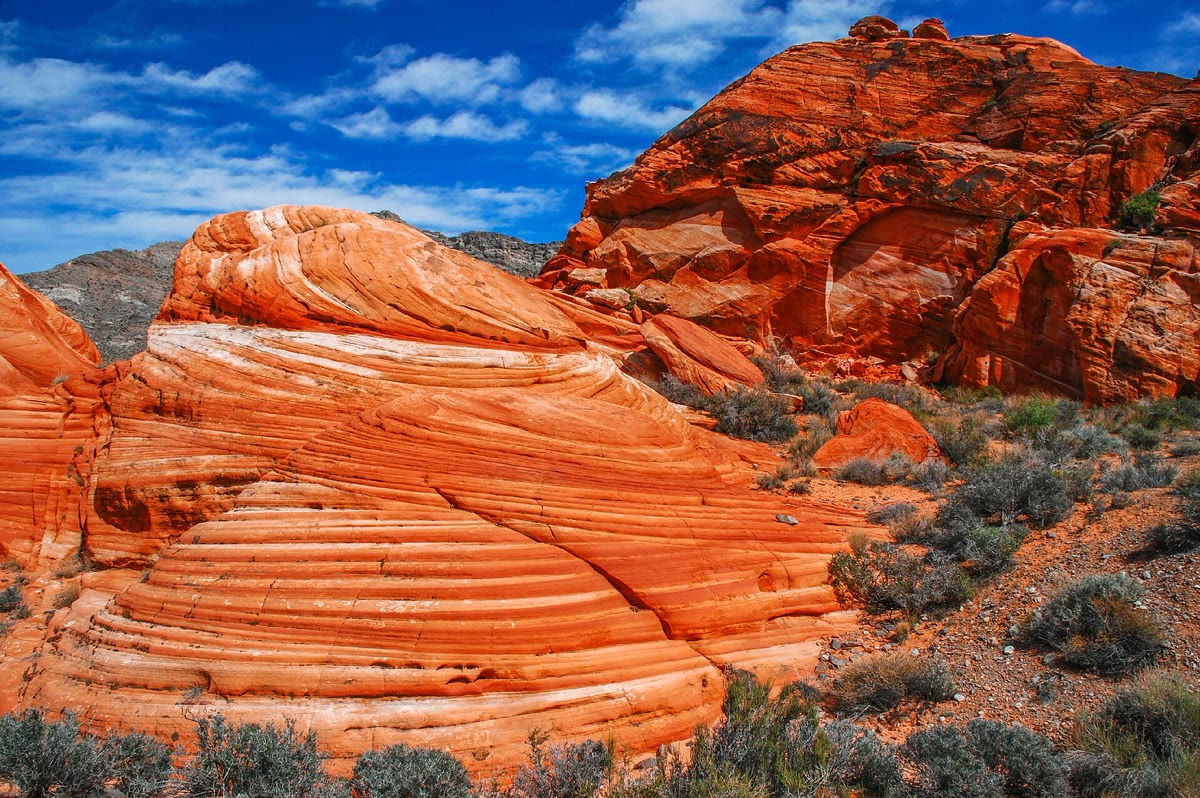
\includegraphics[height=3.6cm]{images/book3/b1-cross-bedding-aztec.jpg}};
\end{tikzpicture}

{\small Kiri: geometri \omterm{def:b1:clastic-sediments:bedform}{bentuk dasar} yang memanjat (skematis, sudut dilebih-lebihkan). Lintasan lembah bergerak sepanjang garis lurus yang miring pada sudut memanjat $\theta$ (garis tebal); di antara dua di antaranya bagian bawah foreset terawetkan, dalam set setebal $T = L\sin\theta$. Kanan: \omterm{def:b1:clastic-sediments:cross-bedding}{perlapisan silang} dalam Batu Pasir Aztec, Muddy Mountains, Nevada: set laminasi miring, masing-masing terpotong di atas oleh permukaan erosi di dasar set berikutnya. Foto Chip Carroon, Biro Pengelolaan Lahan AS, CC~BY-SA~2.0, melalui Wikimedia Commons.}
\label{fig:b1:clastic-sediments:climb}
\end{omfigure}
% ledger: southard:climb, commons:aztec-crossbed

\emph{\omterm{def:b1:clastic-sediments:cross-bedding}{Paleoarus}.} \omterm{def:b1:geological-maps:attitude}{Arah kemiringan} \omterm{def:b1:clastic-sediments:cross-bedding}{perlapisan silang} yang diukur pada \omterm{def:b1:geological-maps:geological-map}{singkapan} tersebar di sekitar arah rerata arus, karena muka lereng \omterm{def:b1:clastic-sediments:bedform}{bukit pasir} dan \omterm{def:b1:clastic-sediments:bedform}{riak} melengkung dan arusnya sendiri berkelana. Rerata mereka diambil sebagai rerata vektor, bukan aritmetik, untuk alasan yang ditunjukkan dalam \cref{prop:b1:field-lab-methods-1:vector-mean}: \omterm{def:b1:spherical-astronomy:horizontal}{azimut} adalah sudut pada lingkaran, dan 350 dan 010 rata-ratanya 000, bukan 180.

\begin{proposition}[Rerata azimut]\label{prop:b1:clastic-sediments:azimuths}
Misalkan $\alpha_1, \ldots, \alpha_N$ adalah \omterm{def:b1:spherical-astronomy:horizontal}{azimut}, diukur searah jarum jam dari utara. Rerata vektor mereka $\bar\alpha$ dan panjang resultan rerata mereka $\bar R$ diberikan oleh
\[
  S = \sum_{i=1}^N \sin\alpha_i, \quad C = \sum_{i=1}^N \cos\alpha_i, \quad
  \bar\alpha = \operatorname{atan2}(S, C), \quad \bar R = \frac{\sqrt{S^2 + C^2}}{N},
\]
dengan $\operatorname{atan2}(S, C)$ adalah sudut yang sinus dan kosinusnya sebanding dengan $S$ dan $C$, diambil antara \ang{0} dan \ang{360}. $\bar R$ terletak antara 0 dan 1, dan bernilai 1 hanya jika semua \omterm{def:b1:spherical-astronomy:horizontal}{azimut} sama.
\end{proposition}

\begin{proof}
Vektor satuan \omterm{def:b1:spherical-astronomy:horizontal}{azimut} $\alpha$, dengan timur sebagai koordinat pertama dan utara sebagai koordinat kedua, adalah $(\sin\alpha, \cos\alpha)$. Jumlah dari $N$ vektor satuan adalah
$(S, C)$, dan arahnya, rerata vektor
(\cref{def:b1:field-lab-methods-1:mean-orientation}), memiliki \omterm{def:b1:spherical-astronomy:horizontal}{azimut} yang sinus dan kosinusnya adalah $S/\sqrt{S^2+C^2}$ dan $C/\sqrt{S^2+C^2}$. Dengan ketidaksamaan segitiga, panjang jumlah dari $N$ vektor satuan paling banyak $N$, dengan kesamaan hanya jika semuanya menunjuk ke arah yang sama.
\end{proof}

\begin{method}[Paleoarus dari perlapisan silang]\label{met:b1:clastic-sediments:palaeocurrent}
\begin{enumerate}
  \item Pada setiap set, ukur \omterm{def:b1:geological-maps:attitude}{arah kemiringan} foreset, dengan memilih permukaan yang menunjukkan \omterm{def:b1:geological-maps:attitude}{kemiringan} sebenarnya (atau ukur \omterm{def:b1:geological-maps:attitude}{jurus} dan \omterm{def:b1:geological-maps:attitude}{kemiringan}).
  \item Ukur posisi perlapisan utama; jika ia miring lebih dari beberapa derajat, putar setiap foreset kembali ke horizontal terhadap \omterm{def:b1:geological-maps:attitude}{jurus} perlapisan (putaran yang dilakukan dengan proyeksi stereografis dalam volume Tahun ke-3).
  \item Hitunglah rerata vektor $\bar\alpha$ dan $\bar R$ dari \omterm{def:b1:geological-maps:attitude}{arah kemiringan} yang telah dikoreksi (\cref{prop:b1:clastic-sediments:azimuths}).
  \item Plot pembacaan sebagai diagram mawar, histogram melingkar \omterm{def:b1:spherical-astronomy:horizontal}{azimut}, untuk melihat apakah mereka membentuk satu kelompok atau dua: arus pasang surut yang berbalik membangun set yang miring ke arah berlawanan, dalam \omterm{def:b1:clastic-sediments:cross-bedding}{perlapisan silang} tulang ikan (herringbone), dan satu rerata menjadi tak bermakna.
\end{enumerate}
\end{method}
% ledger: og:sorting-environments

\emph{Struktur lain.} Beberapa struktur lain mencatat kondisi pengendapan dan arah atas lapisan. \omterm{def:b1:clastic-sediments:turbidite}{Lapisan bergradasi} menghalus ke atas, dari kasar di dasarnya hingga halus di puncaknya, saat butiran mengendap dari arus yang surut, yang paling kasar lebih dulu (\cref{def:b1:clastic-sediments:turbidite}). Retakan lumpur, poligon retakan penyusutan yang diisi oleh lapisan berikutnya, terbentuk ketika lumpur mengering di udara, seperti di dataran pasang surut dan dataran banjir. Cekungan erosi yang dipotong oleh arus ke dalam lumpur di bawahnya, dan diisi oleh pasir di atasnya, terawetkan sebagai cetakan pada dasar lapisan batu pasir, dan bentuknya menunjukkan ke mana arus pergi.
% ledger: og:sorting-environments

\section{Fasies, sungai dan delta}\label{sec:b1:clastic-sediments:rivers-deltas}

Ukuran butir, \omterm{def:b1:clastic-sediments:sorting}{pemilahan}, struktur, fosil dan komposisi bersama-sama membentuk karakter sebuah batuan sedimen, dan geolog memakai satu kata untuk karakter itu.

\begin{definition}[Fasies sedimen, lingkungan pengendapan]\label{def:b1:clastic-sediments:facies}
Sebuah \emph{fasies sedimen}\index{fasies sedimen} adalah sebuah tubuh batuan sedimen yang dibedakan dari yang lain oleh litologinya, ukuran butirnya, struktur sedimennya dan fosilnya, yang semuanya mencerminkan kondisi tempat ia terbentuk. \emph{Lingkungan pengendapan}\index{lingkungan pengendapan} adalah tempat, dengan kondisi fisik, kimia dan biologisnya, tempat sebuah sedimen diletakkan: saluran sungai, dataran banjir, pantai, lereng delta, dasar laut dalam.
\end{definition}
% ledger: og:sorting-environments

Fasies adalah deskripsi, lingkungan adalah interpretasi, dan beberapa lingkungan dapat menghasilkan fasies yang sama: pasir berriak diendapkan di sungai, di dataran pasang surut dan di dasar laut dalam. Interpretasi karena itu bertumpu pada asosiasi fasies dan pada urutan tempat mereka bertumpuk, yang mengikuti pergerakan lingkungan dalam ruang: hukum-hukum umum penumpukan itu, dan model baku setiap lingkungan, menjadi pokok bahasan volume Tahun ke-3. Bab ini menguraikan lingkungan klastik utama dan urutan vertikal yang mengidentifikasinya.

\emph{Sungai menganyam dan berkelok.} Sungai hadir dalam dua gaya utama. Sungai menganyam mengalir dalam banyak saluran yang bercabang dan bertemu kembali di sekitar gosong kerikil dan pasir; sungai menganyam membawa muatan kasar dekat sumbernya, di bawah gunung atau di depan gletser, dan endapannya berupa lembaran kerikil dan pasir kasar berperlapisan silang, dengan sedikit lumpur. Sungai berkelok mengalir dalam satu saluran berliku. Air tercepat mengalir di sepanjang sisi luar setiap tikungan, tempat ia menggerus tebing yang terkikis; di sisi dalam, tempat air paling lambat, pasir diendapkan pada gosong tepi. Meander dengan demikian bermigrasi ke samping, menggerus di satu sisi dan membangun di sisi lain; dataran banjir di luar tepiannya hanya menerima lumpur dari banjir.
% ledger: og:rivers

Urutan gosong tepi mengikuti dari \omterm{def:b1:clastic-sediments:bedform}{bentuk dasarnya}. Di kaki gosong, di air yang paling dalam dan tercepat, arus meninggalkan butiran paling kasar dan membangun \omterm{def:b1:clastic-sediments:bedform}{bukit pasir}; ke atas di sepanjang gosong yang landai air menjadi lebih dangkal dan lebih lambat, pasir lebih halus dan \omterm{def:b1:clastic-sediments:bedform}{bukit pasir} memberi jalan kepada \omterm{def:b1:clastic-sediments:bedform}{riak} (\cref{sec:b1:clastic-sediments:bedforms}); di puncak, gosong menyatu dengan dataran banjir. Ketika tikungan bermigrasi, setiap zona ini bergerak di atas zona di bawahnya, dan lubang bor yang menembus endapan menemukannya bertumpuk: urutan menghalus ke atas dari permukaan erosi hingga lumpur, satu untuk setiap lintasan saluran, yang tebalnya kira-kira sama dengan kedalaman saluran yang membentuknya.

\emph{Delta.} Di tempat sungai masuk ke badan air yang diam, arusnya menyebar dan melambat, dan muatannya dijatuhkan: muatan kasar dekat muara, muatan halus lebih jauh ke luar. Delta tumbuh ke depan, atau berprogradasi, selama sungai memasok lebih banyak sedimen daripada yang dapat dibawa pergi oleh ombak dan pasang surut. Apa yang dilakukan ombak dan pasang surut terhadap pasokan itu menentukan bentuknya.

\begin{definition}[Delta yang didominasi sungai, ombak dan pasang surut]\label{def:b1:clastic-sediments:delta}
Sebuah delta \emph{didominasi sungai}\index{delta didominasi sungai} ketika pasokan sungai mengalahkan ombak dan pasang surut, dan saluran-saluran distributarinya, dibatasi oleh tanggulnya sendiri, membangun jari-jari pasir yang panjang ke laut; ia \emph{didominasi ombak}\index{delta didominasi ombak} ketika ombak mengerjakan ulang pasir yang dibawa ke muara menjadi pantai dan punggung pantai sepanjang pantai yang halus dan melengkung; ia \emph{didominasi pasang surut}\index{delta didominasi pasang surut} ketika arus pasang surut, yang mengalir masuk dan keluar dari muara, membentuk pasirnya menjadi gosong dan punggungan sejajar dengan aliran, dipisahkan oleh saluran berbentuk corong.
\end{definition}
% ledger: og:deltas

\begin{omfigure}
\begin{tikzpicture}[font=\footnotesize, >={Stealth[length=4pt]}]
% meander in plan view (schematic) and the fining-upward log of a point bar
\begin{scope}[yscale=0.8]
  \fill[green!8] (-0.2,-0.4) rectangle (7.2,4.4);
  \draw[omSea!80!black, line width=9pt] plot[smooth, tension=0.7] coordinates {(0,3.6) (1.4,3.7) (2.6,2.8) (2.3,1.4) (3.2,0.5) (4.6,0.8) (5.0,2.2) (5.6,3.4) (7.0,3.5)};
  \draw[omSea!45, line width=7pt] plot[smooth, tension=0.7] coordinates {(0,3.6) (1.4,3.7) (2.6,2.8) (2.3,1.4) (3.2,0.5) (4.6,0.8) (5.0,2.2) (5.6,3.4) (7.0,3.5)};
  % point bars (inside of bends) with scroll lines
  \foreach \r in {0.25,0.45,0.65} {\draw[brown!60!black, densely dotted] (3.45,1.15) ++(200:\r) arc[start angle=200, end angle=340, radius=\r];}
  \fill[brown!25, opacity=0.8] (3.45,1.25) ellipse[x radius=0.55, y radius=0.35];
  \node[align=center] at (3.45,1.95) {gosong tepi\\ (pengendapan)};
  \fill[brown!25, opacity=0.8] (1.75,2.75) ellipse[x radius=0.4, y radius=0.45];
  \node[align=center] at (1.3,1.95) {gosong tepi};
  \draw[red!60!black, thick] (2.9,0.2) .. controls (3.3,0.0) and (4.3,0.15) .. (4.85,0.6);
  \node[red!60!black, anchor=north] at (4.0,0.0) {tebing tergerus (erosi)};
  \draw[->, black!70] (5.9,3.0) -- (6.7,3.15) node[right] {aliran};
  \node[anchor=north west, black!60] at (5.2,1.3) {dataran banjir};
  \node[font=\footnotesize] at (3.5,-0.85) {(a) sebuah meander, dari atas};
\end{scope}
\begin{scope}[xshift=9.2cm, yshift=-0.3cm, yscale=0.8]
  % log: x width = grain size; y = height
  \draw[lith shale] (0,3.6) rectangle (0.8,4.6);
  \draw[lith sandstone] (0,2.6) rectangle (1.2,3.6);
  \draw[lith sandstone] (0,0.6) rectangle (1.7,2.6);
  \draw[lith conglomerate] (0,0) rectangle (2.2,0.6);
  \draw[very thick, red!60!black] (0,0) -- (2.2,0);
  % cross-bed symbols
  \foreach \y in {0.9,1.5,2.1} {\draw[black!70] (0.3,\y) .. controls (0.6,\y+0.05) and (0.9,\y+0.25) .. (1.2,\y+0.4);}
  \foreach \x in {0.2,0.5,0.8} {\draw[black!70] (\x,3.0) -- ++(0.12,0.1) -- ++(0.12,-0.1);}
  \node[anchor=west, align=left] at (2.4,4.1) {lumpur dataran banjir,\\ akar, retakan lumpur};
  \node[anchor=west, align=left] at (2.4,3.1) {pasir halus, laminasi silang\\ riak};
  \node[anchor=west, align=left] at (2.4,1.6) {pasir sedang hingga kasar,\\ perlapisan silang bukit pasir};
  \node[anchor=west, align=left] at (2.4,0.3) {sisa kerikil pada\\ permukaan erosi};
  \draw[->] (-0.35,0) -- (-0.35,4.6) node[above] {atas};
  \draw[<->, black!60] (-0.7,0) -- node[above, rotate=90, font=\scriptsize] {kedalaman saluran} (-0.7,3.6);
  \node[font=\footnotesize] at (1.8,-0.5) {(b) urutan gosong tepi};
\end{scope}
\end{tikzpicture}

{\small (a)~Sebuah meander berkelok (skematis): arus menggerus tebing luar setiap tikungan dan menimbunkan pasir pada gosong tepi di dalamnya; garis-garis lengkung scroll adalah posisi gosong yang berurutan. (b)~Urutan yang ditinggalkan oleh gosong tepi yang bermigrasi, lebar setiap lapisan sebanding dengan ukuran butirnya (skematis). Ia menghalus ke atas, dan tebalnya mencatat kedalaman saluran.}
\label{fig:b1:clastic-sediments:point-bar}
\end{omfigure}
% ledger: og:rivers, southard:phase-diagram

Ketiga kutub itu adalah sudut-sudut segitiga tempat delta mana pun dapat diletakkan menurut kekuatan relatif ketiga proses. Delta kaki-burung dari Mississippi, dengan jari-jarinya yang panjang ke Teluk Meksiko (\cref{ch:b1:erosion-transport}), adalah delta klasik yang \omterm{def:b1:clastic-sediments:delta}{didominasi sungai}; Nil, dengan lengkung pantainya yang halus, adalah delta yang \omterm{def:b1:clastic-sediments:delta}{didominasi ombak}; delta Gangga dan Brahmaputra, yang terbesar di dunia, \omterm{def:b1:clastic-sediments:delta}{didominasi pasang surut}.
% ledger: og:deltas

\begin{omfigure}
\begin{tikzpicture}[font=\footnotesize]
% delta classification triangle (schematic) and the Lena delta from Landsat
\begin{scope}[yscale=0.82]
  \coordinate (R) at (2.6,4.5); \coordinate (W) at (0,0); \coordinate (T) at (5.2,0);
  \fill[omDef!8] (R) -- (W) -- (T) -- cycle;
  \draw[thick] (R) -- (W) -- (T) -- cycle;
  \node[above, align=center] at (R) {\textbf{didominasi sungai}\\ jari-jari memanjang, tanggul};
  \node[below, align=center] at (W) {\textbf{didominasi ombak}\\ punggung pantai halus};
  \node[below, align=center] at (T) {\textbf{didominasi pasang surut}\\ gosong sejajar aliran};
  \fill[omThm] (2.6,2.9) circle[radius=2pt] node[below=1pt] {Mississippi};
  \fill[omThm] (0.75,0.4) circle[radius=2pt] node[above right=0pt] {Nile};
  \fill[omThm] (4.4,0.4) circle[radius=2pt] node[above left=0pt, align=right] {Ganges--\\ Brahmaputra};
\end{scope}
\node[anchor=south west, inner sep=0] at (7.2,-0.9) {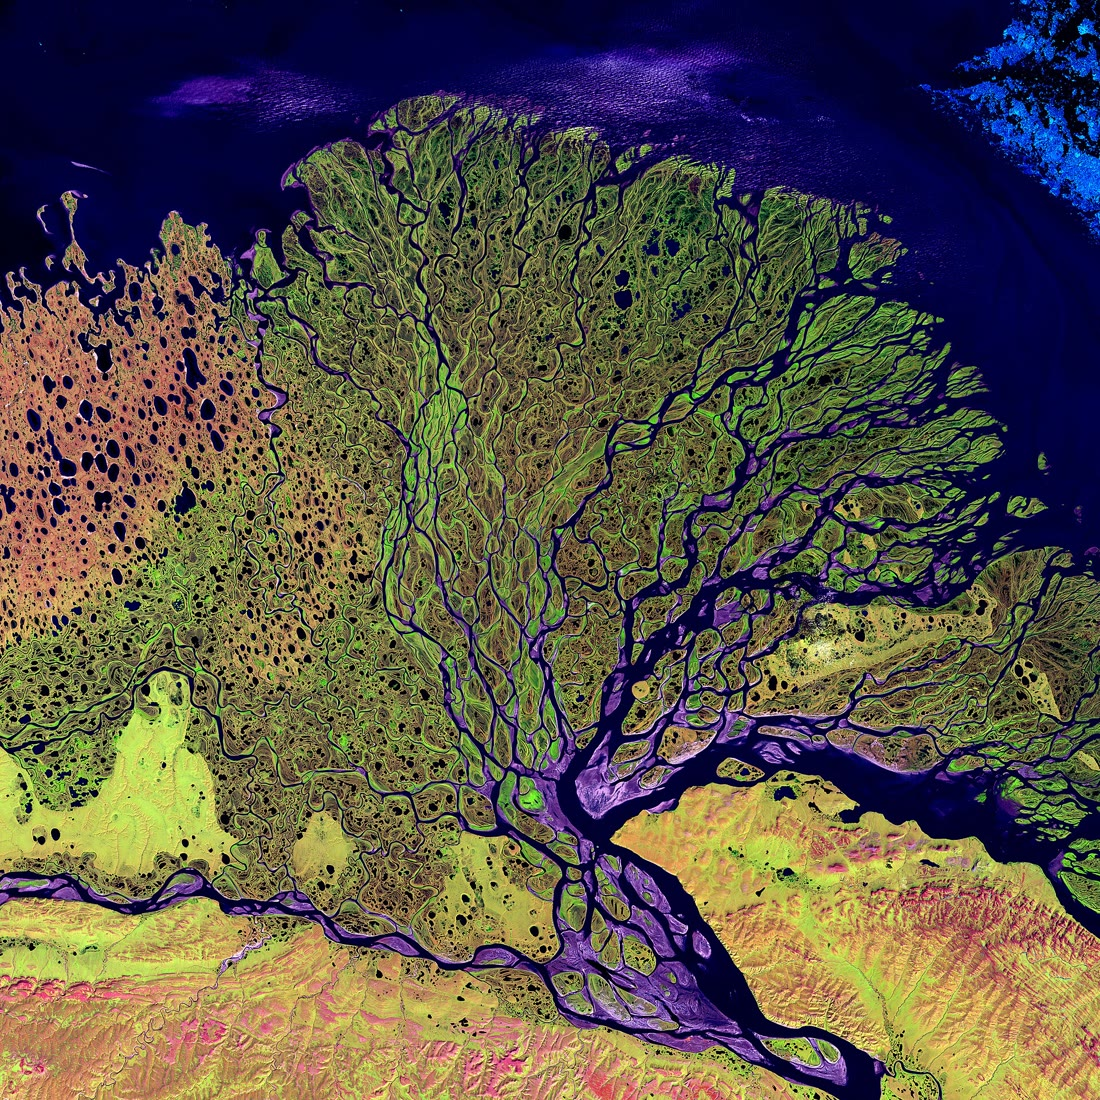
\includegraphics[height=5.2cm]{images/book3/b1-lena-delta.jpg}};
\end{tikzpicture}

{\small Kiri: tiga kutub delta, menurut proses yang membentuknya (skematis; posisi ketiga contoh bersifat indikatif). Kanan: delta Lena, di Siberia, yang menjorok ke Laut Laptev (atas); sungai masuk dari kanan bawah dan terbagi menjadi ratusan distributari. Citra palsu-warna Landsat~7 tanggal 27~Februari 2000, U.S. Geological Survey, domain publik, melalui Wikimedia Commons.}
\label{fig:b1:clastic-sediments:deltas}
\end{omfigure}
% ledger: og:deltas, commons:lena-delta

\emph{Urutan yang mengasar ke atas.} Di depan muara sungai, delta memiliki bagian depan yang landai, bagian depan delta, yang di sisi laut menyatu dengan prodelta, tempat hanya lumpur yang mengendap dari suspensi. Ketika delta berprogradasi, setiap zona ini maju di atas zona di depannya: lubang bor di dataran delta menemukan, dari bawah ke atas, lumpur berlaminasi dari prodelta, kemudian lanau dan pasir yang berselang-seling dari bagian depan delta bawah, lalu pasir berperlapisan silang dari gosong muara, dipotong di atas oleh saluran dataran delta. Urutan itu mengasar ke atas, kebalikan dari gosong tepi, dan tebalnya kira-kira kedalaman air tempat delta itu membangun. Lajunya terkait dengan geometri bagian depan delta.

\begin{proposition}[Progradasi dan akumulasi]\label{prop:b1:clastic-sediments:progradation}
Misalkan suatu bagian depan delta dengan \omterm{def:b1:geological-maps:attitude}{kemiringan} konstan $\alpha$ maju secara horizontal dengan kecepatan $v$ tanpa mengubah bentuk, pada permukaan laut yang konstan. Sebuah titik tetap di bawah bagian depan itu kemudian menerima sedimen dengan laju vertikal
\[
  a = v\,\tan\alpha,
\]
dan urutan bagian depan delta setebal $h$ terakumulasi di sana dalam waktu $h/(v\tan\alpha)$.
\end{proposition}

\begin{proof}
Dalam waktu $\mathrm dt$ bagian depan bergerak maju sejauh $v\,\mathrm dt$. Di titik tetap di bawah permukaan yang miring, permukaan naik sebesar selisih tinggi antara dua titik bagian depan yang berjarak horizontal $v\,\mathrm dt$, yakni $v\,\mathrm dt\,\tan\alpha$, sehingga diperoleh laju itu. Bagian depan melintasi titik itu sementara permukaan naik sebesar $h$, yang memakan waktu $h/a$.
\end{proof}

Bagian depan delta miring landai, sehingga $\tan\alpha$ kecil: bagian depan sebuah delta maju jauh lebih cepat daripada sedimen yang menumpuk di titik mana pun di bawahnya (\cref{exo:b1:clastic-sediments:12}).

\begin{inthelab}[Mendeskripsikan sebuah inti bor]
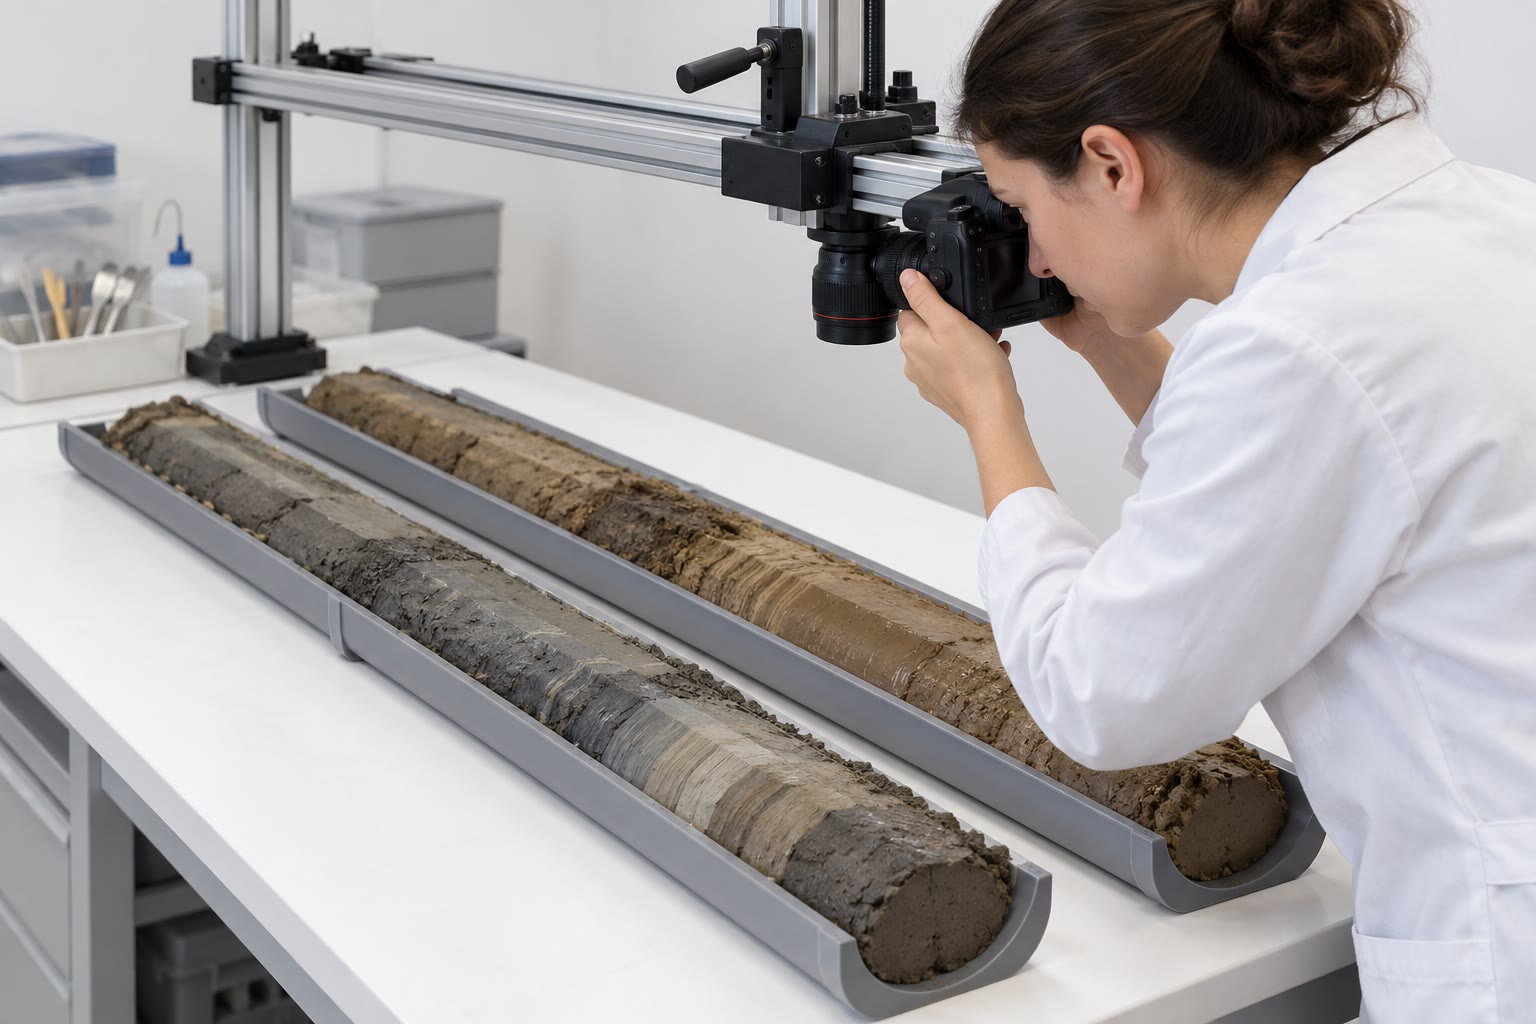
\includegraphics[width=0.3\linewidth]{images/book3/ai/b1-core-lab.jpg}\hfill
\begin{minipage}[b]{0.67\linewidth}
Silinder sedimen atau batuan yang diangkat oleh bor diletakkan dalam baki menurut urutan kedalaman, dibelah memanjang, dan difoto di bawah cahaya merata sebelum mengering dan berubah warna. Ahli sedimentologi kemudian menggambar log inti, meter demi meter: litologi, ukuran butir setiap lapisan (lebar kolom), struktur (\omterm{def:b1:clastic-sediments:cross-bedding}{perlapisan silang}, laminasi, gradasi, liang), \omterm{def:b1:geological-maps:geological-map}{kontak}, tajam atau berangsur, warna dan fosilnya. Sampel diambil untuk analisis ukuran butir dan \omterm{def:b1:field-lab-methods-1:thin-section}{sayatan tipis}. Sebuah inti adalah satu jendela sempit: arah \omterm{def:b1:clastic-sediments:cross-bedding}{perlapisan silang} hilang kecuali inti diorientasikan, dan perluasan lateral lapisan harus berasal dari lubang bor lain.
\end{minipage}

\smallskip
{\small Sebuah inti yang disiapkan untuk difoto di laboratorium sedimen (ilustrasi AI).}
\end{inthelab}

\section{Pantai dan paparan}\label{sec:b1:clastic-sediments:shoreline}

Sepanjang pantai di antara delta, pasir yang dibawa sungai dibentuk oleh ombak dan pasang surut. Pantai adalah pasir yang dikerjakan ulang oleh gelombang sapuan (swash), lapisan air tipis yang naik dan turun di atasnya setelah setiap ombak pecah: butirannya dipindahkan lagi dan lagi, yang halus dibawa ke lepas pantai, dan pasir pantai termasuk yang paling terpilah dan paling membulat dari semua sedimen. Laminasinya, yang diletakkan oleh gelombang sapuan, miring landai ke arah laut. Di banyak pantai rendah pasir membentuk pulau penghalang, punggungan pantai panjang dan \omterm{def:b1:clastic-sediments:bedform}{bukit pasir} yang ditiup angin, yang dipisahkan dari daratan utama oleh laguna, yang tenang dan berbutir halus, dan dihubungkan dengan laut oleh celah pasang surut.

Di tempat pasang surut kuat dan ombak lemah, pantai dihiasi oleh dataran pasang surut, yang tertutup dan tersingkap dua kali sehari. Mereka beralih dari pasir di dekat garis surut, tempat arus paling kuat, ke lumpur di dekat garis pasang tinggi, tempat air tenang membiarkan lempung mengendap; endapan mereka menunjukkan aliran yang berbalik dalam \omterm{def:b1:clastic-sediments:cross-bedding}{perlapisan silang} tulang ikan, pengeringan dalam retakan lumpur, dan selang-seling arus dan air tenang dalam lapisan-lapisan tipis lumpur yang menutupi pasir berriak.

Di lepas pantai, paparan hanya disapu ombak sampai kedalaman yang bertambah seiring ukuran ombak. Di atasnya pasir diayak dan dipindahkan; di bawahnya lumpur mengendap, kecuali selama badai, ketika ombak yang lebih besar mencapai lebih dalam dan mengendapkan lembaran pasir dengan laminasi bergelombang landai yang disebut \omterm{def:b1:clastic-sediments:cross-bedding}{perlapisan silang} gundukan . Urutan paparan dengan demikian sering berselang-seling antara lumpur cuaca cerah dan pasir badai, yang lebih tebal dan lebih kasar ke arah pantai.
% ledger: og:sorting-environments, folk:maturity

\section{Klastik laut dalam}\label{sec:b1:clastic-sediments:deep-sea}

Pasir dan kerikil juga mencapai dasar samudra dalam, ribuan meter ke bawah dan ratusan kilometer dari daratan, dan mereka dibawa ke sana oleh aliran yang tidak pernah dilihat secara utuh oleh siapa pun: arus padat yang sarat sedimen, mengalir menuruni lereng benua di bawah air jernih samudra.

\begin{history}[Kabel di dasar laut, 1929]
Pada 18~November 1929 gempa dengan \omterm{def:b1:earthquake-source:mw}{magnitudo momen} 7.2 melanda lereng benua di selatan Newfoundland, di sepanjang tepi selatan Grand Banks. Longsoran sekitar \qty{200}{km^3} sedimen bergerak di lereng, dan tsunami menewaskan 28 orang di pantai Newfoundland. Dua belas kabel telegraf yang dibentangkan di dasar laut putus, sebagian di beberapa tempat. Yang di dekat episentrum putus seketika; yang lain, lebih jauh ke selatan dan lebih dalam, putus satu demi satu dalam beberapa jam berikutnya, menurut urutan jaraknya menuruni lereng. Pada 1952 Bruce Heezen dan Maurice Ewing, dengan mempelajari waktu-waktu putusnya, menjelaskannya: longsoran telah berubah menjadi \omterm{def:b1:clastic-sediments:turbidite}{arus turbidit} yang mengalir menuruni lereng dan keluar melintasi dataran abisal sejauh lebih dari 480 mil, memutus setiap kabel ketika ia lewat. Dari waktu dan jarak mereka memperkirakan kecepatannya sekitar 50 knot di kaki kontinen bagian atas, tempat lerengnya sekitar \qty{0.5}{\percent}, dan masih 12 knot pada kabel terakhir, sekitar 400 mil dari asalnya. Ketika ia melambat, mereka berpendapat, ia pasti telah mengendapkan \omterm{def:b1:clastic-sediments:turbidite}{lapisan bergradasi} di atas dataran, makin halus ke atas.
\end{history}
% ledger: nrcan:grand-banks, he52:grand-banks

Lima puluh knot adalah \qty{25.7}{m.s^{-1}}, lebih dari \qty{90}{km.h^{-1}}, kecepatan mobil di jalan raya utama; 12 knot adalah \qty{6.2}{m.s^{-1}}; dan 480 mil sekitar \qty{770}{km}. Putusnya kabel juga memberikan kecepatan terukur pertama dari sebuah aliran yang sebelumnya hanya disimpulkan dari endapannya dan dari eksperimen di bak.
% ledger: he52:grand-banks

\begin{definition}[Arus turbidit, turbidit, lapisan bergradasi]\label{def:b1:clastic-sediments:turbidite}
Sebuah \emph{arus turbidit}\index{arus turbidit} adalah arus air yang dibuat lebih padat daripada air di sekitarnya oleh sedimen yang ditahannya dalam suspensi, yang mengalir menuruni lereng di bawah air itu, butiran-butirannya ditahan dalam suspensi oleh turbulensi yang diciptakan oleh geraknya sendiri. Sebuah \emph{turbidit}\index{turbidit} adalah endapan arus turbidit. Sebuah \emph{lapisan bergradasi}\index{lapisan bergradasi} adalah lapisan yang ukuran butirnya menurun dari dasar ke puncaknya.
\end{definition}
% ledger: og:sorting-environments, he52:grand-banks

\omterm{def:b1:clastic-sediments:turbidite}{Arus turbidit} menggerakkan dirinya sendiri: ia mengalir karena suspensinya berat, dan ia mempertahankan suspensinya karena ia mengalir. Di lereng yang curam ia dapat mengambil lebih banyak sedimen dari dasar, menjadi lebih padat dan bertambah cepat; di lereng landai dataran abisal ia melambat, menjatuhkan muatannya dan mati.

\begin{proposition}[Kecepatan arus turbidit]\label{prop:b1:clastic-sediments:turbidity}
Sebuah \omterm{def:b1:clastic-sediments:turbidite}{arus turbidit} dengan ketebalan $h$ dan massa jenis $\rho + \Delta\rho$ mengalir tunak menuruni lereng $S$ di bawah air dengan massa jenis $\rho$. Jika hambatan dasar dan air di atasnya adalah $\tau = \rho\,C_f\,U^2$ per satuan luas, dengan $C_f$ koefisien gesekan tak berdimensi, kecepatan rerata-nya adalah
\[
  U = \sqrt{\frac{\Delta\rho}{\rho}\,\frac{g\,h\,S}{C_f}} .
\]
\end{proposition}

\begin{proof}
Argumennya sama dengan hasil kali kedalaman dan \omterm{def:b1:geological-maps:attitude}{kemiringan}
(\cref{prop:b1:erosion-transport:depth-slope}), dengan berat diganti oleh kelebihan berat. Sebuah kolom arus seluas satuan berat $(\rho +
\Delta\rho) g h$, dan air yang dipindahkannya $\rho g h$: di air sekitarnya, hanya kelebihan $\Delta\rho\,g\,h$ yang menariknya menuruni lereng, dengan
komponen $\Delta\rho\,g\,h\,S$ sepanjangnya. Dalam aliran tunak ini menyeimbangkan
hambatan $\rho C_f U^2$, sehingga $U^2 = (\Delta\rho/\rho)\,g\,h\,S/C_f$.
\end{proof}

Hukum hambatan $\tau = \rho C_f U^2$, kuadrat dalam kecepatan, adalah hukum aliran turbulen dalam hidraulika (buku-buku fisika), dan $C_f$ ditemukan melalui eksperimen. Rumus ini mengabaikan air yang dicampurkan arus ke dalam dirinya sendiri melalui permukaan atasnya, yang mengencerkan dan memperlambatnya. Ia menunjukkan peran ketiga faktor: arus dua kali lebih tebal, atau dua kali lebih padat, atau di lereng dua kali lebih curam, berjalan $\sqrt 2$ kali lebih cepat. Suspensi yang menahan fraksi $c$ dari volumenya sebagai butiran kuarsa memiliki $\Delta\rho/\rho = 1.65\,c$
(\cref{sec:b1:erosion-transport:settling}), kecil kecuali aliran sangat pekat; di sinilah \omterm{def:b1:clastic-sediments:turbidite}{arus turbidit} berbeda dari sungai, di mana seluruh berat air, bukan kelebihan kecil, menggerakkan aliran. Untuk berjalan dengan 50 knot pada 1929 di lereng setengah persen, \omterm{def:b1:clastic-sediments:turbidite}{arus turbidit} membutuhkan hasil kali tebal dan kelebihan massa jenis yang besar (\cref{exo:b1:clastic-sediments:11}).

\emph{Urutan Bouma.} Pada 1962 Arnold Bouma menguraikan urutan internal lapisan batu pasir dari suksesi laut dalam kuno dalam lima divisi, diberi label dari bawah ke atas. A: pasir masif atau bergradasi, sering di atas dasar erosif; B: pasir dengan laminasi sejajar; C: pasir halus dengan laminasi silang \omterm{def:b1:clastic-sediments:bedform}{riak}, sering terlipat (konvolut); D: lanau berlaminasi yang menghalus menjadi lumpur; E: lumpur. Urutan itu dibaca sebagai catatan satu arus yang surut melewati suatu titik: ketika ia melambat, ia pertama-tama menjatuhkan butiran terkasarnya sekaligus, lalu membangun dasar datar atas, kemudian \omterm{def:b1:clastic-sediments:bedform}{riak}, lalu membiarkan lanau dan lempung mengendap. Urutan lengkap jarang: divisi-divisi atasnya sering tererosi oleh arus berikutnya, dan jauh dari sumber, tempat arus lemah, divisi-divisi bawahnya tidak ada.
% ledger: og:sorting-environments, shanmugam:bouma

\begin{omfigure}
\begin{tikzpicture}[font=\footnotesize]
% Bouma sequence: log (schematic) and a labelled photograph
\begin{scope}
  \draw[lith shale] (0,4.0) rectangle (0.7,4.8);
  \draw[lith shale] (0,3.3) rectangle (0.9,4.0);
  \draw[lith sandstone] (0,2.2) rectangle (1.3,3.3);
  \draw[lith sandstone] (0,1.2) rectangle (1.6,2.2);
  \draw[lith sandstone] (0,0) rectangle (2.0,1.2);
  \draw[very thick, red!60!black] (0,0) .. controls (0.6,-0.12) and (1.4,0.1) .. (2.0,0);
  \foreach \y in {1.4,1.6,1.8,2.0} {\draw[black!70] (0.1,\y) -- (1.5,\y);}
  \foreach \x in {0.15,0.5,0.85} {\draw[black!70] (\x,2.55) .. controls (\x+0.12,2.75) .. (\x+0.3,2.6);}
  \foreach \y in {3.45,3.6,3.75,3.9} {\draw[black!60] (0.1,\y) -- (0.8,\y);}
  \foreach \x/\y in {0.4/0.3, 0.9/0.5, 1.4/0.25, 0.6/0.8, 1.2/0.9} {\fill[black!60] (\x,\y) circle[radius=0.06];}
  \node[anchor=west] at (2.2,4.4) {E \quad lumpur};
  \node[anchor=west] at (2.2,3.65) {D \quad lanau berlaminasi ke lumpur};
  \node[anchor=west] at (2.2,2.75) {C \quad laminasi silang riak};
  \node[anchor=west] at (2.2,1.7) {B \quad laminasi sejajar};
  \node[anchor=west] at (2.2,0.6) {A \quad pasir bergradasi};
  \node[anchor=west, red!60!black] at (2.2,-0.15) {dasar erosif, tanda dasar};
  \draw[->] (-0.3,0) -- (-0.3,4.8) node[above] {atas};
\end{scope}
\node[anchor=south west, inner sep=0] at (6.9,-0.3) {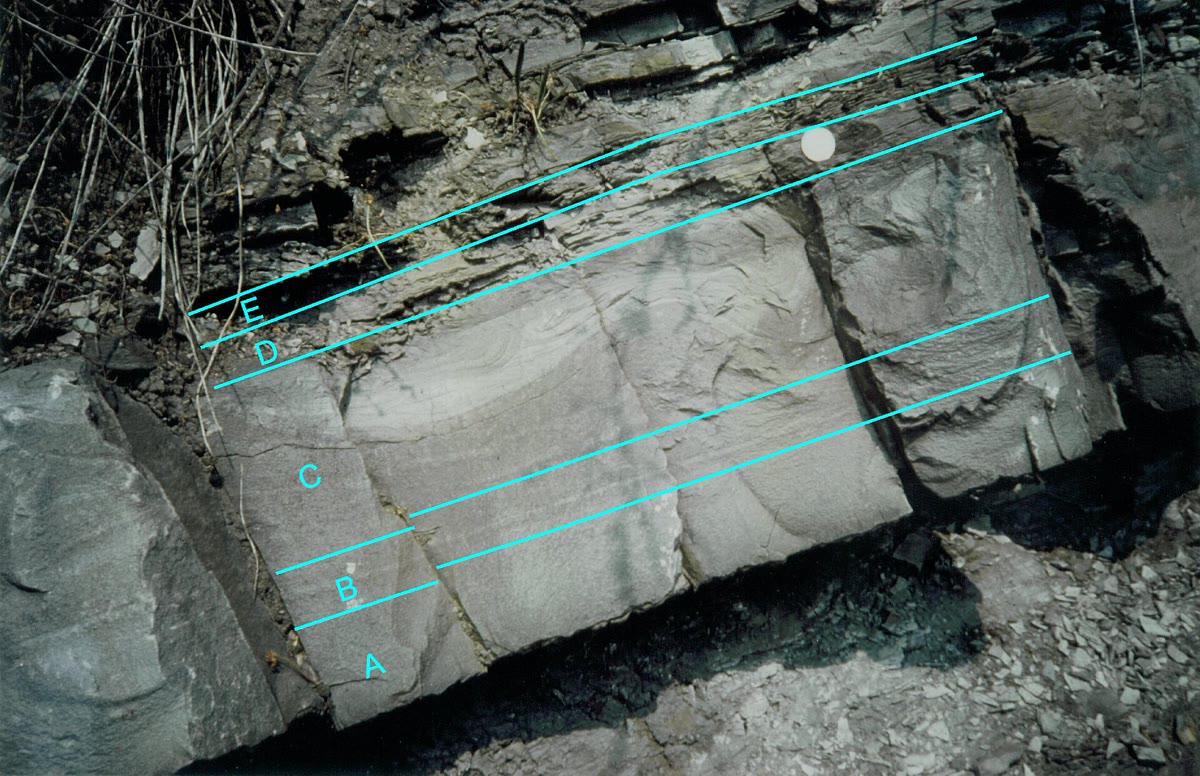
\includegraphics[height=5.2cm]{images/book3/b1-turbidite-bouma.jpg}};
\end{tikzpicture}

{\small Kiri: lima divisi urutan Bouma, lebar setiap divisi sebanding dengan ukuran butirnya (skematis). Kanan: lapisan \omterm{def:b1:clastic-sediments:turbidite}{turbidit} Devon Atas di Becke-Oese, Jerman, dengan divisi A hingga E yang ditandai oleh fotografer; koin memberi skala. Foto Jo Weber, CC~BY-SA~3.0, melalui Wikimedia Commons.}
\label{fig:b1:clastic-sediments:bouma}
\end{omfigure}
% ledger: og:sorting-environments, shanmugam:bouma, commons:bouma-becke-oese

Urutan Bouma menjadi model baku \omterm{def:b1:clastic-sediments:turbidite}{turbidit}, dan ribuan batu pasir laut dalam kuno ditafsirkan dengannya. Penafsiran itu diperdebatkan: arus yang mengalir sepanjang lereng, arus pasang surut laut dalam dan gelombang internal juga membangun pasir berriak dan berlaminasi, dan sebagian ahli sedimentologi berpendapat bahwa banyak lapisan yang dibaca sebagai \omterm{def:b1:clastic-sediments:turbidite}{turbidit}, termasuk sebagian dari yang berada di wilayah tipenya, diendapkan oleh aliran lain. Sedikit \omterm{def:b1:clastic-sediments:turbidite}{arus turbidit} yang pernah diamati di samudra modern, sementara \omterm{def:b1:clastic-sediments:turbidite}{turbidit} kuno dihitung dalam ribuan.
% ledger: shanmugam:bouma

Tidak semua klastik laut dalam adalah \omterm{def:b1:clastic-sediments:turbidite}{turbidit}. Arus kontur, arus lambat dan dalam yang mengikuti kontur lereng benua, mengerjakan ulang sedimen lereng menjadi endapan memanjang yang halus, yaitu kontourit. Dan jauh dari benua, tempat baik \omterm{def:b1:clastic-sediments:turbidite}{arus turbidit} maupun arus kontur tidak mencapai, dasar laut hanya menerima apa yang mengendap dari air di atasnya: cangkang plankton dan debu halus yang diterbangkan angin, sedimen pelagis dalam bab berikutnya (\cref{ch:b1:chemical-biogenic-sediments}).
% ledger: og:sorting-environments

\section{Latihan}

\begin{exercise}[$\star$]\label{exo:b1:clastic-sediments:1}
Ubahlah ke satuan phi diameter-diameter \qty{0.18}{mm}, \qty{0.75}{mm},
\qty{3}{mm}, \qty{0.012}{mm} dan \qty{150}{mm}, hingga dua desimal, dan sebutkan kelas masing-masing (\cref{tab:b1:clastic-sediments:classes}).
% ledger: folk:wentworth-classes
\end{exercise}

\begin{exercise}[$\star$]\label{exo:b1:clastic-sediments:2}
Kurva kumulatif sebuah pasir sungai memberi $\varphi_5 = 0.62$, $\varphi_{16} =
1.05$, $\varphi_{50} = 1.71$, $\varphi_{84} = 2.43$ dan $\varphi_{95} = 2.98$. Hitunglah rerata grafisnya, dalam satuan phi dan dalam milimeter, dan simpangan baku grafis inklusifnya, dan sebutkan ukuran serta \omterm{def:b1:clastic-sediments:sorting}{pemilahannya}.
% ledger: folk:graphic-measures, folk:sorting-classes
\end{exercise}

\begin{exercise}[$\star$]\label{exo:b1:clastic-sediments:3}
\omterm{def:b1:clastic-sediments:bedform}{Riak} setinggi \qty{2}{cm} bermigrasi \qty{1}{cm} per menit di atas dasar pasir kuarsa dengan porositas \num{0.4}. Dengan \cref{prop:b1:clastic-sediments:migration}, hitunglah volume \omterm{def:b1:erosion-transport:load}{muatan dasar} per satuan lebar, dalam \si{m^2.s^{-1}}, dan massa kuarsa ($\qty{2650}{kg.m^{-3}}$) yang terbawa melewati satu meter puncak dalam sehari.
% ledger: hom:quartz
\end{exercise}

\begin{exercise}[$\star$]\label{exo:b1:clastic-sediments:4}
Satu knot adalah satu mil laut, \qty{1852}{m}, per jam. (a)~Ubahlah ke meter per detik kecepatan 50 dan 12 knot yang diperkirakan untuk \omterm{def:b1:clastic-sediments:turbidite}{arus turbidit} 1929. (b)~Berapa lama arus pada 12 knot menempuh \qty{100}{km}? (c)~Ubahlah 480 dan 400 mil ke kilometer (satu mil adalah \qty{1.609}{km}).
% ledger: he52:grand-banks
\end{exercise}

\begin{exercise}[$\star\star$]\label{exo:b1:clastic-sediments:5}
(a)~Dengan menggunakan persentil distribusi normal yang diberikan dalam bukti \cref{prop:b1:clastic-sediments:normal}, hitunglah simpangan baku grafis $(\varphi_{84} - \varphi_{16})/2$ dan perkiraan $(\varphi_{95} - \varphi_5)/3.3$ untuk distribusi normal dengan simpangan baku $\sigma$. (b)~Mengapa keduanya dapat berbeda untuk sedimen sungguhan? Jenis sedimen mana yang paling membuat keduanya berbeda?
\end{exercise}

\begin{exercise}[$\star\star$]\label{exo:b1:clastic-sediments:6}
Sebuah endapan \omterm{def:b1:clastic-sediments:bedform}{riak} memanjat menunjukkan set setebal \qty{1.5}{cm}, diukur tegak lurus terhadap batasnya, yang dibuat oleh \omterm{def:b1:clastic-sediments:bedform}{riak} berjarak \qty{15}{cm}. (a)~Hitunglah sudut memanjatnya. (b)~Jika \omterm{def:b1:clastic-sediments:bedform}{riak} bergerak \qty{0.5}{cm} per menit, dengan laju berapa dasar dinaikkan, dalam sentimeter per jam? (c)~Apa yang dikatakan laju seperti itu tentang aliran?
% ledger: southard:climb
\end{exercise}

\begin{exercise}[$\star\star$]\label{exo:b1:clastic-sediments:7}
Enam \omterm{def:b1:geological-maps:attitude}{arah kemiringan} \omterm{def:b1:clastic-sediments:cross-bedding}{perlapisan silang}, yang telah dikoreksi untuk \omterm{def:b1:geological-maps:attitude}{kemiringan} lapisan, terbaca 350, 020, 005, 340, 015 dan 030. (a)~Hitunglah rerata aritmetiknya. (b)~Hitunglah rerata vektornya dan $\bar R$. (c)~Jelaskan perbedaannya.
\end{exercise}

\begin{exercise}[$\star\star$]\label{exo:b1:clastic-sediments:8}
Tiga batu pasir diperiksa dalam \omterm{def:b1:field-lab-methods-1:thin-section}{sayatan tipis}. A memiliki \qty{12}{\percent} matriks lempung dan butiran kuarsa, \omterm{def:b1:rock-forming-minerals:groups}{feldspar} serta pecahan batuan yang bersudut. B memiliki \qty{2}{\percent} lempung, $\sigma_I = 0.40\,\varphi$ dan butiran kuarsa dengan kebulatan \num{2.2} pada skala Folk. C tidak memiliki lempung, $\sigma_I =
0.30\,\varphi$, butiran kuarsa dengan kebulatan \num{3.6}, dan \qty{98}{\percent} kuarsa. Sebutkan \omterm{def:b1:clastic-sediments:maturity}{kematangan tekstur} masing-masing, dan usulkan \omterm{def:b1:clastic-sediments:facies}{lingkungan pengendapan} untuk setiap batu pasir.
% ledger: folk:maturity
\end{exercise}

\begin{exercise}[$\star\star$]\label{exo:b1:clastic-sediments:9}
(a)~Hitunglah bilangan Froude aliran sedalam \qty{0.3}{m} pada
\qty{1.5}{m.s^{-1}}, dan sungai sedalam \qty{2}{m} pada \qty{1.0}{m.s^{-1}} ($g
= \qty{9.81}{m.s^{-2}}$). (b)~Pada kedalaman berapakah aliran sebesar \qty{1.5}{m.s^{-1}} mencapai bilangan Froude 1, dan kecepatan berapakah yang dibutuhkan sungai sedalam \qty{2}{m}? (c)~Mengapa antidun umum pada lapisan air yang mengalir dari pantai, dan jarang di sungai-sungai besar?
% ledger: southard:ripples-dunes
\end{exercise}

\begin{exercise}[$\star\star\star$]\label{exo:b1:clastic-sediments:10}
Analisis ayakan sebuah pasir memberi, dalam kelas-kelas phi utuh dari $-1$ hingga $5\,\varphi$: 2, 8, 30, 40, 15 dan 5 persen berat. (a)~Dengan metode momen, hitunglah rerata dan simpangan baku dalam satuan phi, dan sebutkan \omterm{def:b1:clastic-sediments:sorting}{pemilahannya}. (b)~Bangunlah kurva kumulatif, bacalah $\varphi_5$, $\varphi_{16}$, $\varphi_{50}$, $\varphi_{84}$ dan $\varphi_{95}$ dengan interpolasi linear, dan hitunglah $M_z$ dan $\sigma_I$. (c)~Bandingkan.
% ledger: folk:graphic-measures, folk:sorting-classes
\end{exercise}

\begin{exercise}[$\star\star\star$]\label{exo:b1:clastic-sediments:11}
Ambil $C_f = 0.003$ dalam \cref{prop:b1:clastic-sediments:turbidity}. (a)~Sebuah \omterm{def:b1:clastic-sediments:turbidite}{arus turbidit} setebal \qty{50}{m}, dengan kelebihan massa jenis \qty{2}{\percent}, mengalir menuruni lereng sebesar \num{0.005}: hitunglah kecepatannya, dalam meter per detik dan dalam knot. (b)~Hasil kali tebal dan kelebihan massa jenis relatif apakah yang akan memberi 50 knot pada 1929 di lereng yang sama? (c)~Arus yang sama seperti pada (a) mencapai lereng sebesar \num{0.001}: hitunglah kecepatan barunya, jika tidak ada yang lain berubah. Apa yang terjadi pada muatannya?
% ledger: he52:grand-banks
\end{exercise}

\begin{exercise}[$\star\star\star$]\label{exo:b1:clastic-sediments:12}
Sebuah sungai mengirim \qty{50}{Mt} sedimen setahun ke deltanya, dan \qty{70}{\percent} darinya diendapkan pada bagian depan delta selebar \qty{100}{km} yang membangun ke dalam air sedalam \qty{30}{m}. Endapan itu memiliki massa jenis curah \qty{2000}{kg.m^{-3}}. (a)~Berapa volume yang ditambahkannya setiap tahun? (b)~Jika volume ini mengisi seluruh kedalaman air di sepanjang lebar bagian depan, seberapa cepat bagian depan maju? (c)~Dengan \omterm{def:b1:geological-maps:attitude}{kemiringan} bagian depan delta \ang{0.5}, dengan laju berapa sedimen menumpuk di suatu titik tetap di bawah bagian depan, dan dalam berapa tahun urutan yang mengasar ke atas terbentuk di sana?
\end{exercise}

\section{Masalah: membaca inti dari sebuah delta}

\begin{problem}[{Soal akhir pekan --- lubang bor menembus delta kuno, dari ukuran butir
hingga arah sungai-sungainya}]
\label{pb:b1:clastic-sediments:1}
% values: calc/ch21.py; the borehole, its beds, ages and readings are invented
Sebuah lubang bor memotong \qty{24}{m} batu pasir dan batulumpur yang diendapkan oleh delta kuno. Ahli geologi mendeskripsikan empat satuan, dari dasar ke atas, dan menganalisis sampel dari setiap satuan.

\smallskip
\begin{center}\small
\begin{tabular}{@{}l>{\raggedright\arraybackslash}p{4.2cm}ccccc@{}}
\hline
unit (kedalaman dari dasar) & deskripsi & $\varphi_5$ & $\varphi_{16}$ & $\varphi_{50}$ & $\varphi_{84}$ & $\varphi_{95}$ \\
\hline
1 (0--8 m) & batulumpur abu-abu berlaminasi & 4.2 & 5.0 & 6.6 & 8.4 & 9.6 \\
2 (8--16 m) & batulanau dan batu pasir yang berselang-seling & 1.9 & 2.4 & 3.4 & 4.6 & 5.5 \\
3 (16--21 m) & batu pasir berperlapisan silang & 0.9 & 1.25 & 1.8 & 2.35 & 2.7 \\
4 (21--24 m) & batu pasir berkerikil, dasar erosif & $-1.8$ & $-0.8$ & 0.9 & 2.1 & 2.9 \\
\hline
\end{tabular}
\end{center}

\medskip
\noindent\textbf{Bagian I --- Ukuran butir.}
\begin{enumerate}
  \item Hitunglah rerata grafis $M_z$ setiap satuan, dalam satuan phi dan dalam milimeter.
  \item Hitunglah simpangan baku grafis inklusif $\sigma_I$ setiap satuan.
  \item Sebutkan kelas ukuran rerata dan \omterm{def:b1:clastic-sediments:sorting}{pemilahan} setiap satuan.
  \item Satuan mana yang paling terpilah? Mengapa gosong muara akan lebih terpilah daripada lumpur prodelta?
  \item Dengan interpolasi linear antara $\varphi_{50}$ dan $\varphi_{84}$, perkirakan persentase partikel berukuran lempung (lebih halus dari $8\,\varphi$) pada satuan~1. Apa yang dikatakannya tentang arus tempat ia diendapkan?
  \item Mengapa kurva kumulatif satuan~4 begitu menyebar, meskipun ia adalah pasir saluran?
\end{enumerate}

\medskip
\noindent\textbf{Bagian II --- Suksesinya.}
\begin{enumerate}[resume]
  \item Jelaskan bagaimana ukuran rerata berubah dari satuan~1 ke satuan~3. Apakah suksesi itu menghalus atau mengasar ke atas?
  \item Tafsirkan satuan 1, 2 dan 3 sebagai bagian dari sebuah delta. Zona delta mana yang berada di lokasi ketika masing-masing diendapkan?
  \item Apa yang ditunjukkan oleh penumpukan ketiga satuan tentang pergerakan delta?
  \item Setidaknya, sedalam apa air tempat delta itu membangun, dan mengapa?
  \item Satuan~4 memiliki dasar erosif dan lebih kasar daripada satuan~3. Tafsirkan ia.
  \item Apakah gosong tepi akan memberikan suksesi yang sama? Jelaskan.
\end{enumerate}

\medskip
\noindent\textbf{Bagian III --- Seberapa cepat delta maju?}
Dua lapisan tipis abu vulkanik, di dasar satuan~1 dan di puncak satuan~2, diberi tarikh; keduanya berjarak \num{4000}~tahun.
\begin{enumerate}[resume]
  \item Hitunglah laju akumulasi rerata di antara kedua abu, dalam milimeter setahun.
  \item Bagian depan delta miring pada \ang{0.5}. Dengan \cref{prop:b1:clastic-sediments:progradation}, hitunglah kecepatan ia maju, dalam meter setahun.
  \item Seberapa jauh bagian depan maju selama \num{4000}~tahun?
  \item Berapa lama 21 meter satuan 1 hingga 3 membutuhkan waktu untuk terakumulasi di lokasi itu, pada laju ini?
  \item Mengapa laju akumulasi di delta tidak sama di setiap tempat pada waktu yang sama?
\end{enumerate}

\medskip
\noindent\textbf{Bagian IV --- Ke mana sungai-sungai mengalir?}
Pada batu pasir berperlapisan silang dari satuan~3, yang tersingkap di \omterm{def:b1:geological-maps:geological-map}{singkapan} terdekat tempat lapisannya mendatar, diukur dua belas \omterm{def:b1:geological-maps:attitude}{arah kemiringan} foreset: 352, 010, 025, 004, 338, 017, 031, 359, 012, 046, 006 dan 344.
\begin{enumerate}[resume]
  \item Hitunglah rerata aritmetik dari dua belas bacaan itu. Apakah itu bermakna?
  \item Hitunglah jumlah $S$ dan $C$ dalam \cref{prop:b1:clastic-sediments:azimuths}.
  \item Hitunglah panjang resultan rerata $\bar R$. Apakah bacaan-bacaan itu konsisten?
  \item Ke arah umum manakah delta itu membangun, dan di mana daratannya?
  \item Mengapa \omterm{def:b1:geological-maps:attitude}{arah kemiringan} harus diputar jika lapisannya miring, dan terhadap sumbu apa?
  \item Apakah arus pasang surut dapat membangun \omterm{def:b1:clastic-sediments:cross-bedding}{perlapisan silang} ini? Seperti apa diagram mawarnya?
  \item Hingga derajat terdekat, berapakah \omterm{def:b1:spherical-astronomy:horizontal}{azimut} \omterm{def:b1:clastic-sediments:cross-bedding}{paleoarus} rerata dari batu pasir berperlapisan silang satuan~3?
\end{enumerate}
\end{problem}
